\documentclass[a4paper,11pt,abstract=on,thesis,twoside]{report}
% \documentclass[a4paper,11pt,abstract=on]{report}
\usepackage[T1]{fontenc}
\usepackage[utf8]{inputenc}
\usepackage{lmodern}
\usepackage{mathptmx}
\usepackage[page]{appendix}
\usepackage{listings}
\usepackage{color}
\usepackage{pdfpages}
\usepackage{lipsum}
\usepackage{float}
\usepackage{textcomp}
\usepackage{bookmark}
\usepackage[english]{babel}
\usepackage{csquotes}
\usepackage{caption}
\usepackage{subcaption}
\usepackage{fancyhdr}
\usepackage{amsmath}
\usepackage{xcolor}
\usepackage[inner=35mm,outer=20mm]{geometry}
\usepackage[style=apa,citestyle=apa,backend=biber,hyperref=true,apabackref=true]{biblatex}
\usepackage{hyperref}
\usepackage{doi}

\DeclareLanguageMapping{english}{english-apa}

\addbibresource{final_report/bibliography.bib}
% \setkomafont{disposition}{\normalfont\bfseries}

\definecolor{mygreen}{rgb}{0,0.6,0}
\definecolor{mygray}{rgb}{0.5,0.5,0.5}
\definecolor{mymauve}{rgb}{0.58,0,0.82}

\lstset{frame=tb,
	aboveskip=3mm,
	belowskip=3mm,
	backgroundcolor=\color{white},   % choose the background color; you must add \usepackage{color} or \usepackage{xcolor}; should come as last argument
	basicstyle={\footnotesize\ttfamily},    % the size of the fonts that are used for the code
	breaklines=true,                 % sets automatic line breaking
	captionpos=b,                    % sets the caption-position to bottom
	commentstyle=\color{mygreen},    % comment style
	columns=flexible,
	keepspaces=true,                 % keeps spaces in text, useful for keeping indentation of code (possibly needs columns=flexible)
	keywordstyle=\color{blue},       % keyword style
	language=Python,                 % the language of the code
	numbers=left,                    % where to put the line-numbers; possible values are (none, left, right)
	numberstyle=\tiny\color{mygray}, % the style that is used for the line-numbers
	numbersep=0pt,
	rulecolor=\color{black},         % if not set, the frame-color may be changed on line-breaks within not-black text (e.g. comments (green here))
	showspaces=false,                % show spaces everywhere adding particular underscores; it overrides 'showstringspaces'
	showstringspaces=false,          % underline spaces within strings only
	showtabs=false,                  % show tabs within strings adding particular underscores
	stepnumber=1,                    % the step between two line-numbers. If it's 1, each line will be numbered
	stringstyle=\color{mymauve},     % string literal style
	tabsize=2,	                     % sets default tabsize to 2 spaces
	postbreak=\mbox{\textcolor{red}{$\hookrightarrow$}\space}, % line breaks with arrows
}

\renewcommand{\lstlistingname}{Code}
\renewcommand{\lstlistlistingname}{List of Code Blocks}

\title{
	{Evaluation of a Haskell Web Framework}\\
	{\large Aston University}\\
	{\large BSC Computer Science}
}
\author{Junaid Ali Rasheed}

\pagestyle{fancy}

\begin{document}
\pagenumbering{roman}


\maketitle

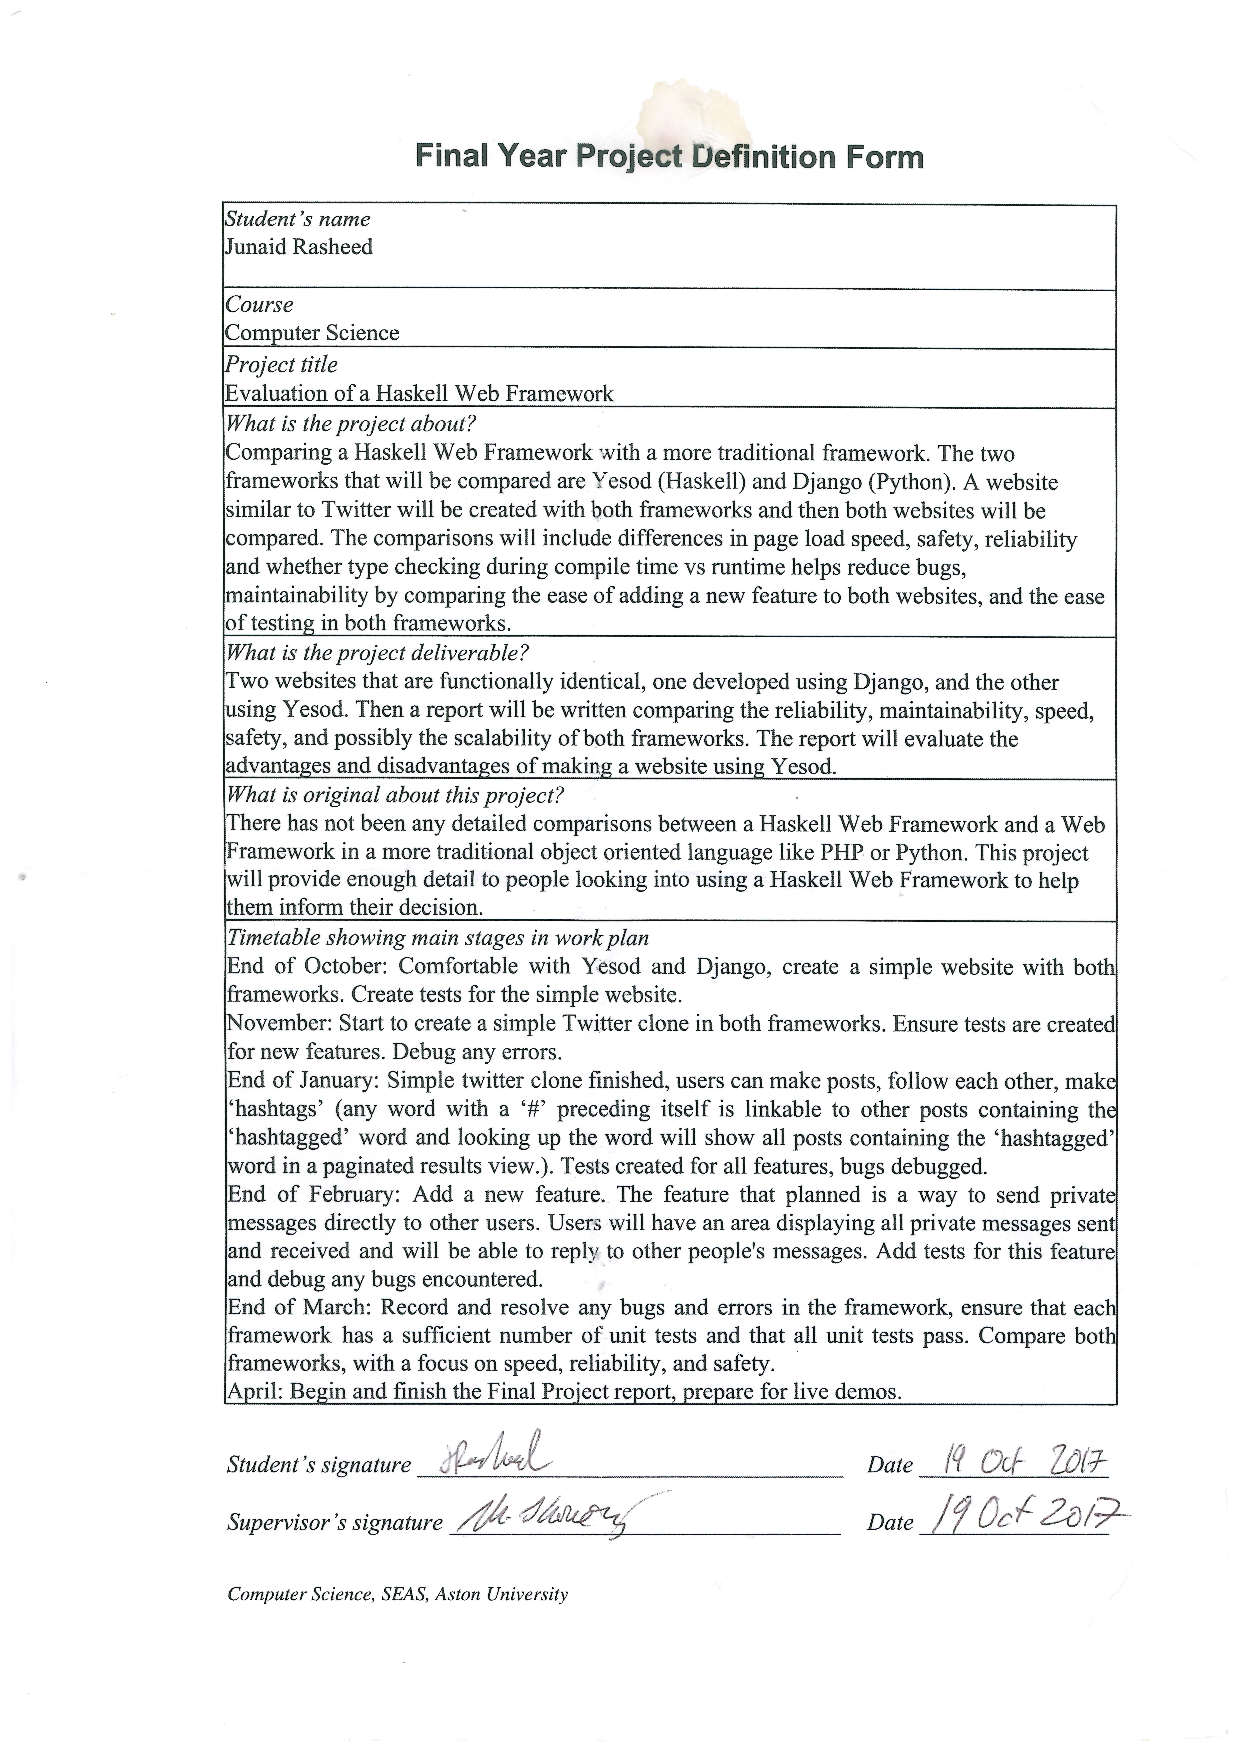
\includepdf[pages=-]{pdf_documents/Final_Year_Project_Definition_Form_Signed.pdf}

\tableofcontents
\listoffigures
\lstlistoflistings

\begin{abstract}
\lipsum[1-3]
\end{abstract}

\pagenumbering{arabic}

\chapter{Introduction}

In this report, we will compare two web frameworks, one written in Haskell and another, more
popular framework, written in a typical object oriented language. To perform the evaluation,
a functionally identical website was created in both frameworks.

One issue that individuals face when looking into Haskell Web frameworks is the lack of
detailed comparisons between these frameworks and more traditional frameworks that these
individuals likely have experience in. This report will provide an in-depth look at the
advantages and disadvantages of choosing to use a Haskell Web Framework, and will help
these individuals come to an informed decision on whether or not a Haskell Web Framework is
best for them.

\section{The Chosen Frameworks}

Yesod is a fully featured and modular web framework written in Haskell. Yesod claims to use
features of the Haskell language to provide a fast, modular, and type safe web framework. By
choosing Yesod as the web framework for the Haskell language, we will be able to determine
whether or not Haskell's type safety, referential transparency, and lazy compiling is an advantage
or a disadvantage for web developers.

\begin{quote}
Yesod attempts to ease the web development process by playing to the strengths of the Haskell 
programming language. Haskell’s strong compile-time guarantees of correctness not only encompass 
types; referential transparency ensures that we don’t have any unintended side effects. Pattern 
matching on algebraic data types can help guarantee we’ve accounted for every possible case. 
By building upon Haskell, entire classes of bugs disappear. \parencite[Introduction]{yesodBook}
\end{quote}

Django is a Python Web Framework. Django, like Yesod, is a ``batteries included'' web framework,
``instead of having to open up the language to insert your own power (batteries), you just have
to flick the switch and Django does the rest.'' \parencite{djangoBookReasons}. I chose Django
for a number of reasons

\begin{itemize}
  \item ``Batteries included'', like Yesod
  \item Modular, like Yesod
  \item Python is now more common than PHP, second only to Node.js \parencite{djangoBookReasons}
\end{itemize}

The Django and Yesod web frameworks have a similar set of features. This ensured that we could
make a functionally identical site in both of these frameworks with a similar 
amount of effort. This enables us to make a fair comparison between Django and Yesod, enabling
us to come to a conclusion on whether a Haskell web framework may be a good choice for a 
developer rather than a more tradition web framework.

\section{The Report}

The rest of this report will discuss any pieces of work similar to this project, the process of
writing the code for both frameworks, including any preparation that had to be done, and a detailed
evaluation of the websites that were produced. The evaluation will compare page load speeds,
the reliability and maintainability of the websites, the ease of writing new code, the ease of
debugging issues, the features including in each framework's test suite, and whether the static typing
and type safety of the Haskell language help or hinder the process of developing a website.
\chapter{Background}
\label{chap:Background}

In this chapter, we will discuss previous work and research pertaining
to Haskell web frameworks and any real-world sites built using a Haskell
web framework.

\section{Similar Previous Work}

Looking through scientific journals, online articles, and blog posts,
you can find many individuals documenting their experiences and performing
reviews of Haskell Web Frameworks. For example, in the IEEE Internet Computing
journal, \citeauthor{snapFramework} have written an article giving an overview
of Snap. According to the article, snap is a simple web framework written
in Haskell where programming is done at a similar level of abstraction
to Java servlets. The article instructs the reader on how to install Snap, 
walks the reader through some sample code, and shows a quick comparison
between Snap and other major web frameworks. The comparison is a benchmark
of each framework, recording the amount of time it takes for each framework
to respond to a request. The benchmark results can be seen in Figure 
~\ref{fig:snapBenchmark}. \parencite{snapFramework}

\begin{figure}[H]
    \centering
    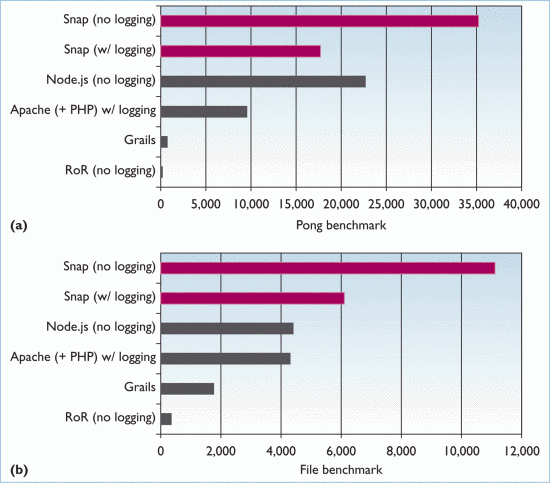
\includegraphics[width=0.7\textwidth]{final_report/pics/snapBenchmark.png}
    \caption{Snap and other frameworks, values are in requests per second \\ \textcopyright{} \citeyear{snapFramework} IEEE}
    \label{fig:snapBenchmark}
\end{figure}

Figure ~\ref{fig:snapBenchmark} shows the results of two benchmarks, one where a server
responded to a request by sending the string "pong", and another that records how fast
a server can send a 49 kilobyte image. As you can see in the
graph, for the file benchmark, the Snap framework was faster than all other frameworks.
Snap was only beaten by Node.js in the Pong benchmark when logging was turned on.
Turning logging off dramatically increased the performance of Snap, resulting in
Snap being 55\% faster than Node.js in the Pong benchmark. \parencite{snapFramework}

So, from the research done by \citeauthor{snapFramework}, we can see that Haskell
web frameworks can be significantly faster than more traditional web frameworks.
This is because Haskell uses the Glasgow Haskell Compiler (GHC). GHC compiles
Haskell programs into native machine code, ensuring high performance, especially
for concurrent programs such as web servers. Because of this, any Haskell web framework
that uses GHC, including Yesod, will serve requests faster than most traditional
web frameworks. \parencite{ghcSite}

\citeauthor{haskellWebComparison} published a blog post on his website with the
title \citetitle{haskellWebComparison}. In the post, \citeauthor{haskellWebComparison}
provides a quick comparison between some popular Haskell Web Frameworks, including
Yesod and Snap. The comparisons include the installation process of each framework,
the way they handle routing -- i.e. pointing a URL to a piece of code that will 
produce a response, and the quality of documentation for each framework. \parencite{haskellWebComparison}

At the end of his comparison, \citeauthor{haskellWebComparison} found that Yesod
was the best framework for his use case. One of the reasons for his choice was
because of the great documentation available for Yesod. The creator of Yesod
has written a book, \citetitle{haskellBook}, that is very comprehensive. The book
is available for free on the Yesod website. The amount of detail contained in this
book is also one of the reasons the Yesod web framework was chosen for this
project. \parencite{haskellWebComparison,yesodBook}

In \citetitle{beginnerYesod}, \citeauthor{beginnerYesod} discusses his experiences
in using Yesod as a beginner to the Haskell programming language. He mentions
the depth and thoroughness of the Yesod book when learning Yesod. However, when
making an actual website, he came across difficulties when trying to implement
features that required the use of functions not in the book. The author had
to check the documentation of the functions on Hackage, a Haskell package archive.
On Hackage, most functions contain a type signature and normally a one line
description. The author mentions how the type signatures would probably be
enough for experienced Haskell developers to work out how to use a function
but, as a beginner, founding out how a function works using types was much more
difficult. Because of this, the author had to spend a lot of time fixing type
errors. \parencite{beginnerYesod}

When first starting the project, I personally experienced the same issues described
in \citeauthor{beginnerYesod}'s blog post. I was not very good at reading the type
signatures available on Hackage, resulting in spending a lot of time fixing
unmatched type errors when trying to use functions not documented in the book.
However, as I became more experienced in Yesod and Haskell, these problems
became more and more rare as my understanding of Haskell type signatures increased.

\section{Real World Haskell Sites}

Some readers will be concerned about whether or not a Haskell web framework like
Yesod is ready for production websites. This is a valid concern considering the
relatively small amount of Haskell programmers when compared to mainstream 
programming languages. Readers will be pleased to know, however, that there
are some high traffic sites that are built using the Yesod web framework.

Freckle, previously known as Front Row Education, is an education
platform that provides a service to almost 10 million students \parencite{frontrowName}. 
In 2015, Freckle migrated their site to the Yesod web framework and have been 
using it ever since. \citeauthor{frontrow}, the CTO of Freckle, wrote an article
on his experience of using Yesod for a high traffic website. \parencite{frontrow}

In his article, \citeauthor{frontrow} states that the reason they chose a Haskell
Web Framework was because of the low resource usage and the ability to make
quick iterations that the Haskell language gives you. The article also discusses
how static typing saves time when writing unit tests. The developers at Freckle
did not have to deal with checking for null exceptions, mismatched types, and
other common bugs that are annoying to deal with. Spending less time dealing with
dynamic typing gives developers more time in implementing their features. The
modularity of Yesod also allows Freckle to reuse complex code, reducing potential
mistakes by developers, reducing the amount of code that needs to be written,
and allowing code to be updated quickly without the need to repeat changes. All
of these advantages allow developers to be more efficient and write fewer bugs. \parencite{frontrow}

However, there are some issues that the Freckle team came across during their migration.
Haskell builds are normally quite slow, as all external libraries used have to be
compiled during the build process. \citeauthor{frontrow} mentions that builds took
5-10 minutes on their most powerful machines. The author does mention that the team
could improve their build process by, for example, caching built files. The testing
suite caused problems for the team because when a test fails, they could not determine
which condition caused the failure when a test block has multiple conditions. The issue,
however, was reported to developers behind the testing library and the current
version of the testing suite does not have the issue mentioned in the article. The
lack of documentation for some functions also caused some frustration to the development
team, especially for the more junior developers who could not rely on type signatures. \parencite{frontrow}

When Freckle switched their main API to Yesod, their CPU usage rose to 95\%. This issue
did not occur during testing and profiling, in fact, the Freckle team were the first to
experience this particular issue. This is one issue when using a relatively niche language
like Haskell, you have to be comfortable with the idea that you may be the first person
to experience a particular issue. With other popular frameworks like Django, any issue
you discover has most likely been found and fixed by other members of the community.

Despite these issues, Freckle decided to stick with Yesod due to the advantages of the
Haskell compiler and the fact that the issues they experienced with regards to documentation
and build time are improving. And although the community is small, you can almost
always find help by asking on the StackOverflow or Google Groups pages or by visiting
the \#haskell-beginners IRC channel, an online chat room where developers new to Haskell
can quickly and easily get help from some more experienced developers.

\chapter{Preparation}
\label{chap:Preparation}

In this chapter, we will discuss the work that needed to be done before work could
be started on developing websites in Yesod and Django.

\section{Planning the Website}

Before any work was done, a plan was created that indicated the features the
website should contain to ensure that the each framework is tested and
evaluated fairly. The website to be created was a twitter
clone with the following features: a home page, authentication, a profile page,
ability to post a message, ability to post `tagged' messages (any words with
a preceding `\#' becomes link that leads to a search page),
ability to search for messages and users, and an ability to follow other users.
All features implemented would also have unit tests implemented using the
testing tools available in each framework. After each site is feature complete,
a new feature, the ability to message other users, should be implemented.

Implementing these features allows us to test page load speed by navigating
to certain web pages. We can evaluate how the static type checking and type safety features of 
Haskell affects reliability when compared to dynamic type checking in Python. Testing
all of our implemented features allows us to fairly evaluate the
test suites included with each framework. Implementing a new feature once each
site is feature complete will also allow us to test the maintainability of
each framework.

By planning the website before any work was done, there was a clear vision of
what the website should look like. This allowed development to focus on implementing
the specified features rather than trying to design new features while developing
at the same time, ensuring that functionally identical websites are created in both
frameworks that can be fairly compared and evaluated.

\section{Learning the Frameworks}

Even after the planning was completed for both sites, before any development could
be done, the basics of each framework must be learned. This ensures that code
produced follows the latest standards of each framework, the built-in features
of each framework that may help with development are understood and used appropriately,
and code produced is of a high standard, maintainable, and readable.

\subsection{Learning Django}

Because of previous experience with Python and other object oriented web frameworks, 
Django was learned quickly by going through the official Django tutorials and 
documentation.

The Django tutorials themselves were straight forward for someone who has 
experience in Python and other web frameworks. The tutorials walk you through
installing Django and creating your own app. In Django, an app resides in a project
and is a web application that performs some function. An example of an app could be
a web blogging system. A Django project is a collection of apps and configuration
settings for a particular website. After completing the Django tutorials, work
on the planned website was begun. \parencite{djangoIntroDocs}

\subsection{Learning Yesod}

Coming from an object oriented background, it was not trivial to start using
a functional programming language like Haskell. Before development with the
Yesod framework could be started, the Haskell language had to be learned to
an adequate level.

To help with learning Haskell, the book \citetitle{haskellBook} \parencite{haskellBook}
was used. This book walks the reader through learning the Haskell language beginning
with the fundamentals. Reading through several chapters of the book gives
the reader a basic understanding of programming with Haskell, allowing the reader
start learning Yesod itself, referring to the book to understand more
advanced concepts as you come across them.

To learn Yesod, the book \citetitle{yesodBook} \parencite{yesodBook}, 
written by the person who wrote Yesod, was used. The book goes through all of the
features of the Yesod framework in an easy to understand manner. After
reading the book, development on the planned website using the Yesod
framework was started.

\section{The Evaluation}

Once the website was feature complete on both frameworks, a series of experiments
were ran to compare the features that we planned to test during the planning phase.
The raw data of these experiments can be found in the appendix and an evaluation
of these results are discussed in the next chapter.

\chapter{Deliverables}
\label{chap:Deliverable}

This chapter will go through the work that was produced as a result of this
project. We will take a look at the website, examples of code for both frameworks,
and how we tested both frameworks.

\section{The Website - Wire}

Most of the features that we planned for were implemented in the final version
of the website. The website was named `Wire' and users can create an account,
post messages, follow other users, see user messages, post tagged
messages, and search for other messages and users. The following subsections
contain pictures of the website produced. The pictures taken are of the Yesod
website but the Django site is functionally identical, with only a few minor styling
differences.

\subsection{The Home Page}

\begin{figure}[H]
	\centering
	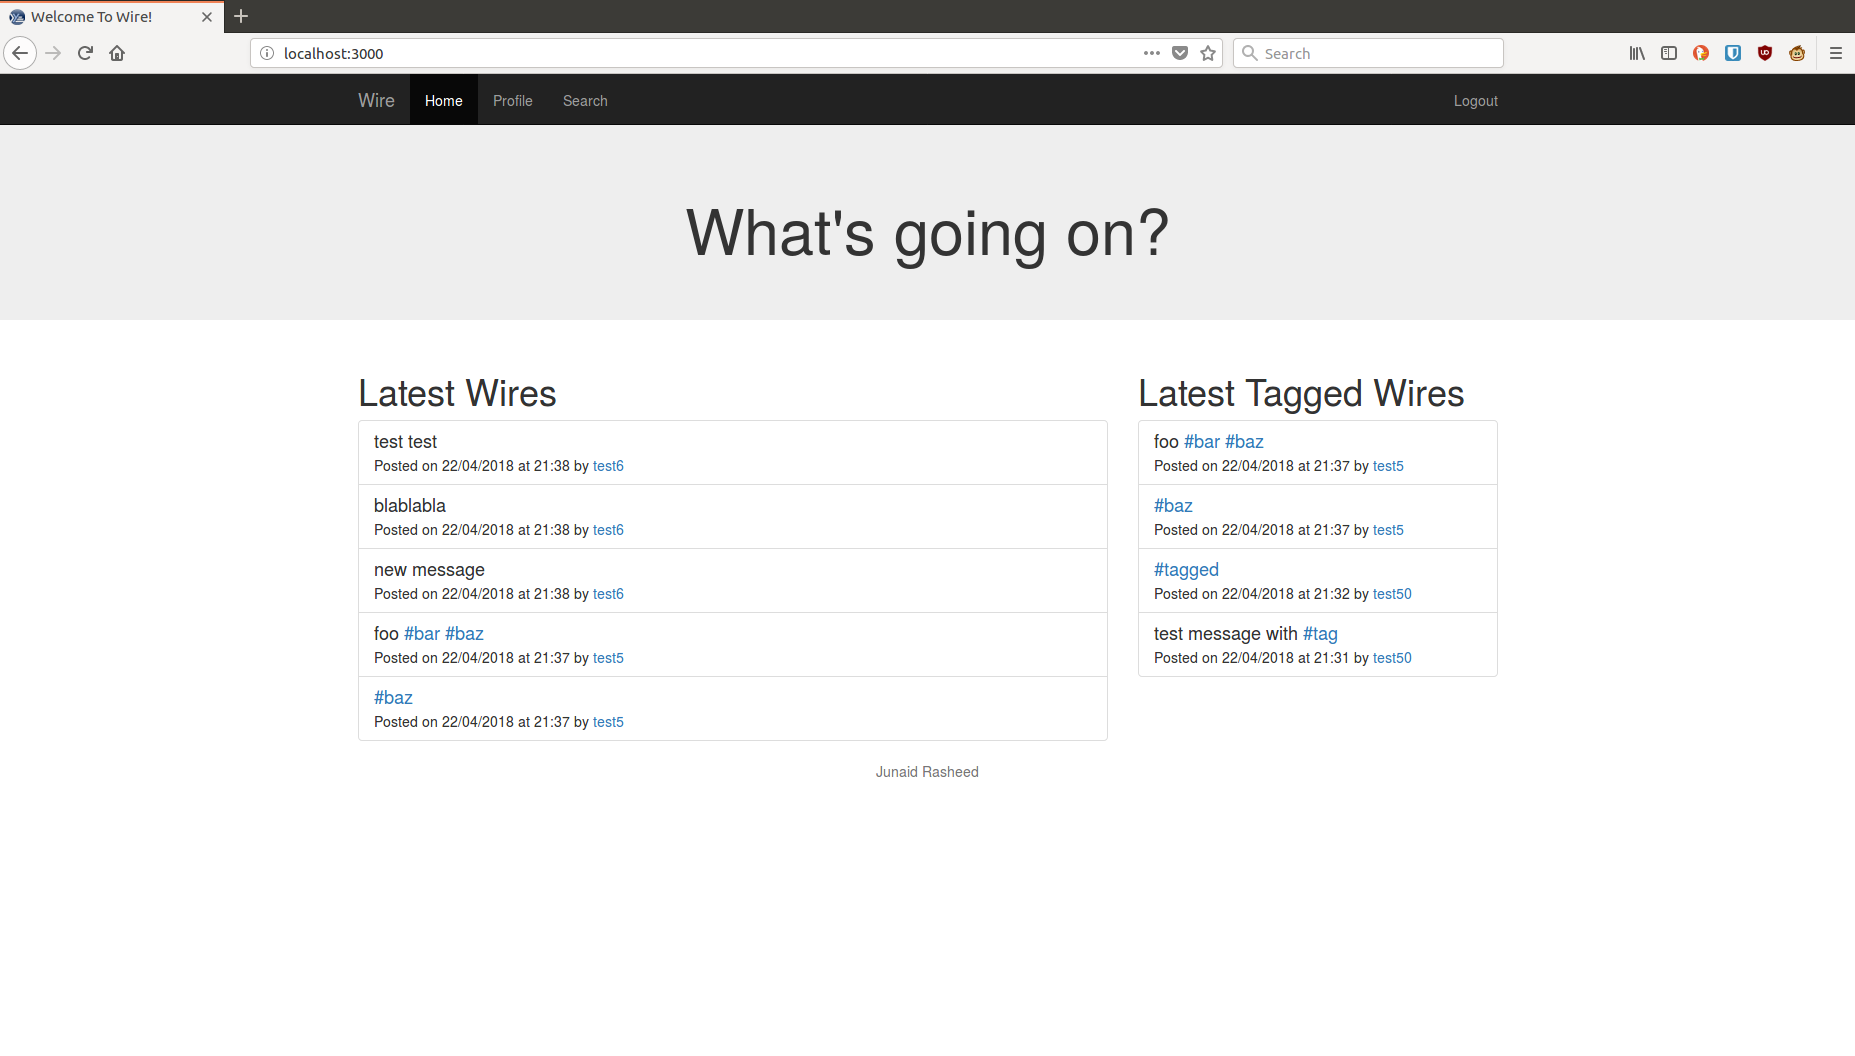
\includegraphics[width=0.7\textwidth]{final_report/pics/home.png}
	\caption{The home page}
	\label{fig:wireHome}
\end{figure}

The home page is the first page the user sees when they access the website.
The home page contains the latest messages posted by users on the website,
with a separate list for tagged messages. Messages that contain tags are links
that take the user to the search page. There is a navigation bar at the top of
the home page. This navigation bar is present on all pages. When a user is not
logged in, the navigation bar allows the user to access the login and signup pages.
Once logged in, the user can use the navigation bar to access their profile page
or to logout.

\subsection{Authentication}

\begin{figure}[htb]
	\centering
	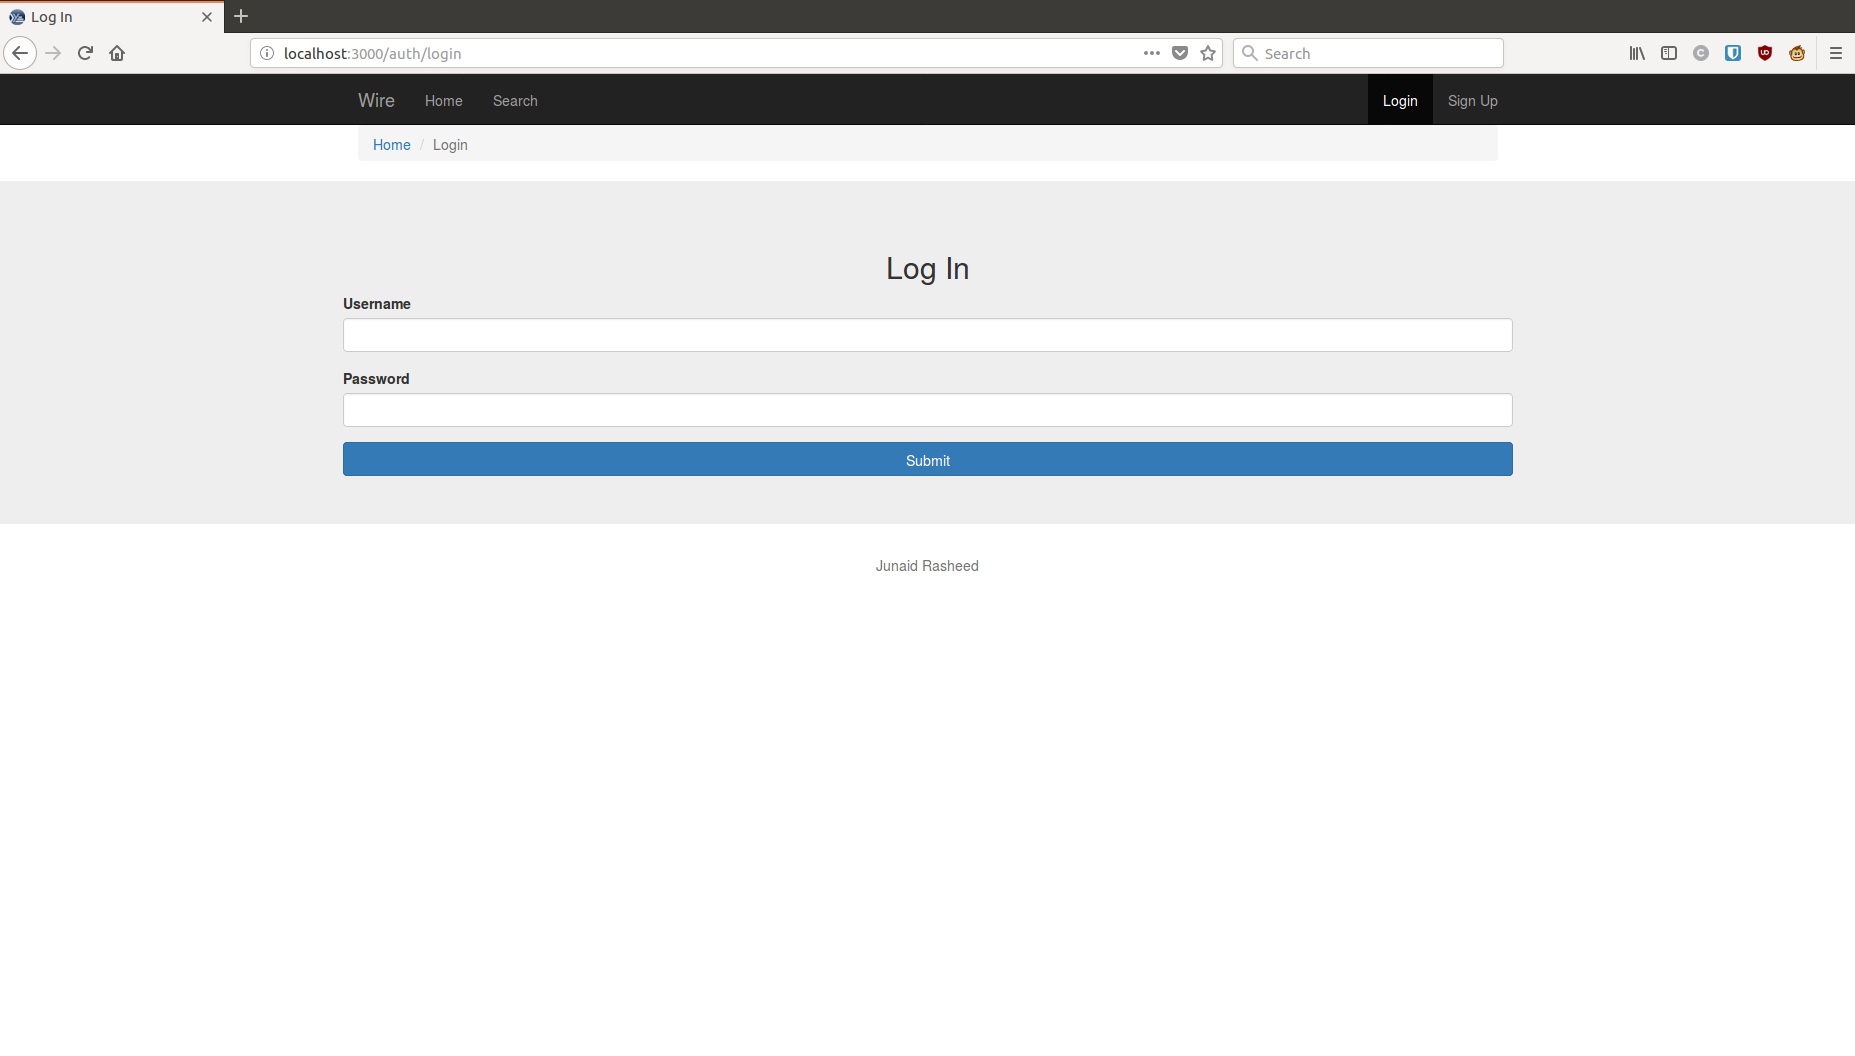
\includegraphics[width=0.7\textwidth]{final_report/pics/login.png}
	\caption{The login page}
	\label{fig:wireLogin}
\end{figure}

\begin{figure}[htb]
	\centering
	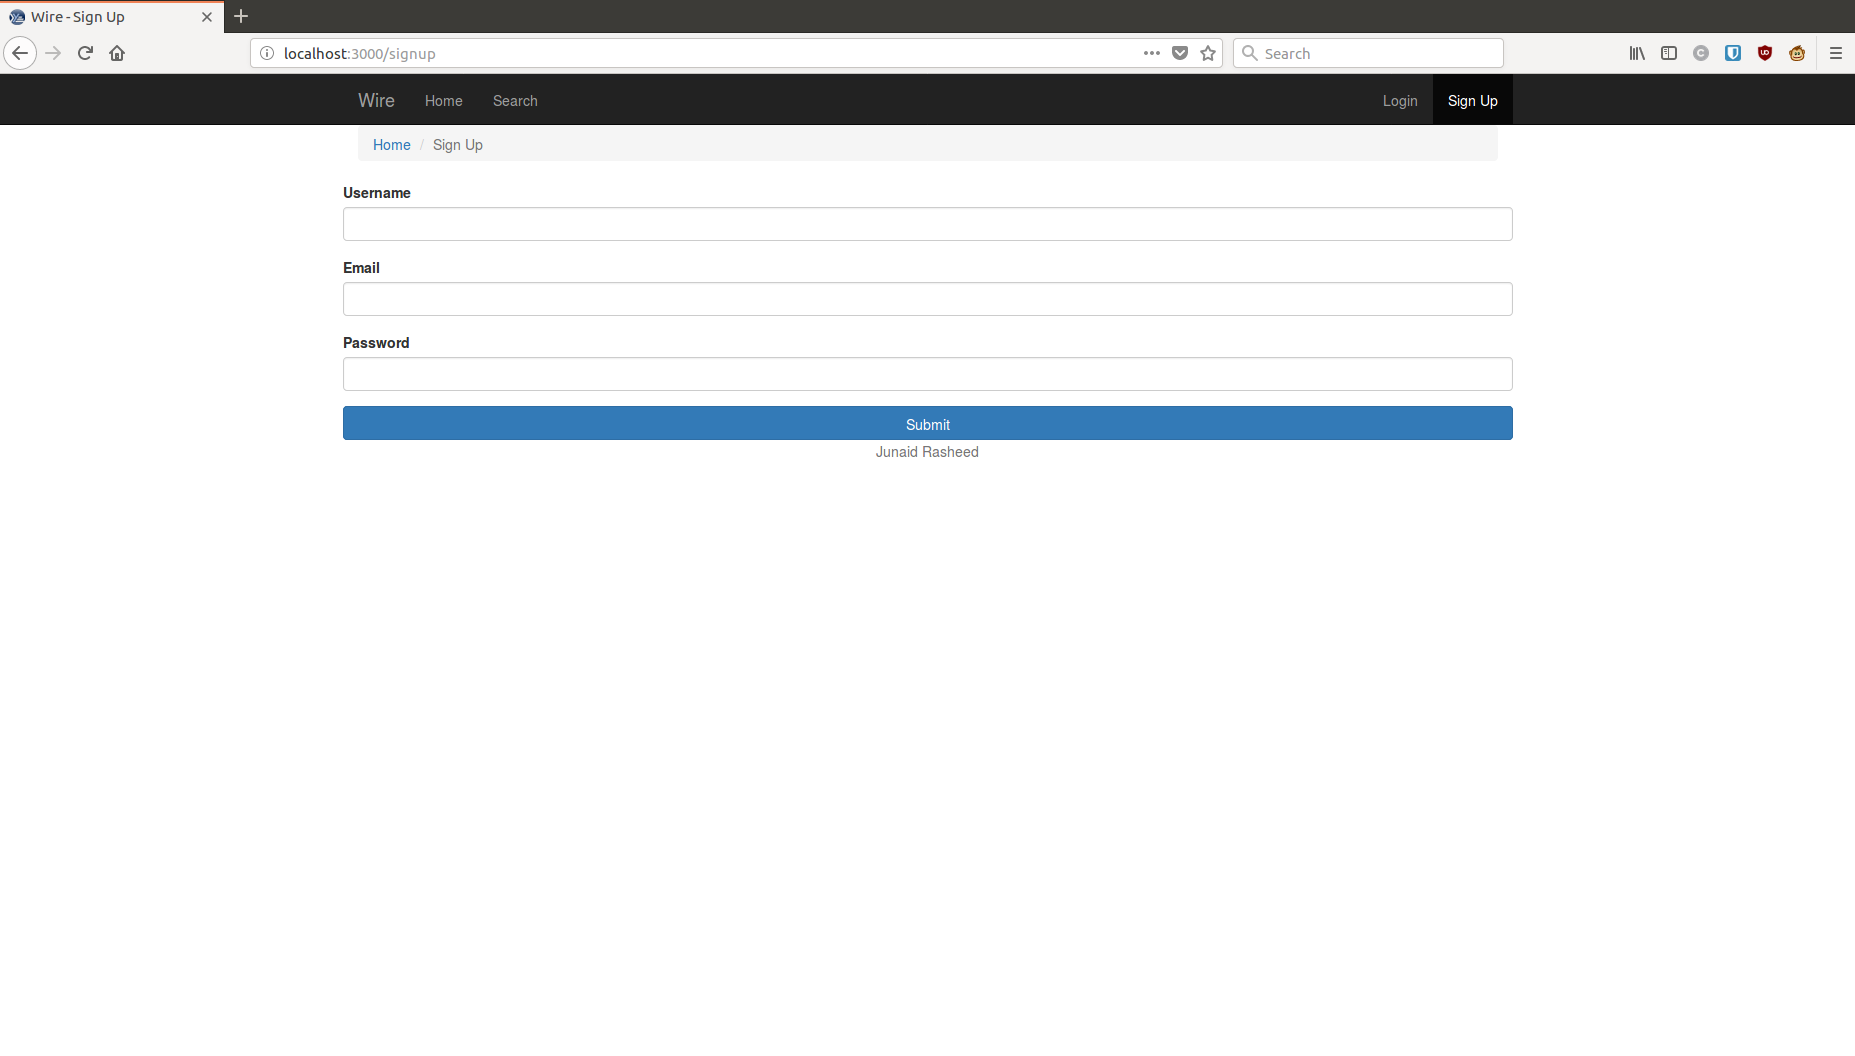
\includegraphics[width=0.7\textwidth]{final_report/pics/signup.png}
	\caption{The signup page}
	\label{fig:wireSignup}
\end{figure}

The authentication functionality of this website includes signing up and
logging in using a web page, and logging out using a button in the navigation
bar. In figure ~\ref{fig:wireSignup}, you can see that signing up requires
a username, e-mail, and password. The username and e-mail must be unique.
Users are shown a warning message if they try to sign up with details that
are already taken. Once a user signs up, their details are stored in the
database, with the password being hashed and salted to ensure that it is
stored safely.

When logging in, you only need to supply a username and password, as you can
see in figure ~\ref{fig:wireLogin}. This is because the username is a unique
identifier, we can use it to determine which user to log in as. When the username
and password is submitted, we look up the username in the database, encrypt the
password, and see if the encrypted password matches the one stored in the database. 
If there is a match, the user is authenticated and redirected to the home page. 
If there is an issue, the user is redirected back to the login page with an 
appropriate error messages.

Once the user is logged in, they can use the log out button which is present
on the top right of the navigation bar. Clicking this button immediately logs
the user out and they are redirected to the home page.

\subsection{User Profiles}

\begin{figure}[H]
	\centering
	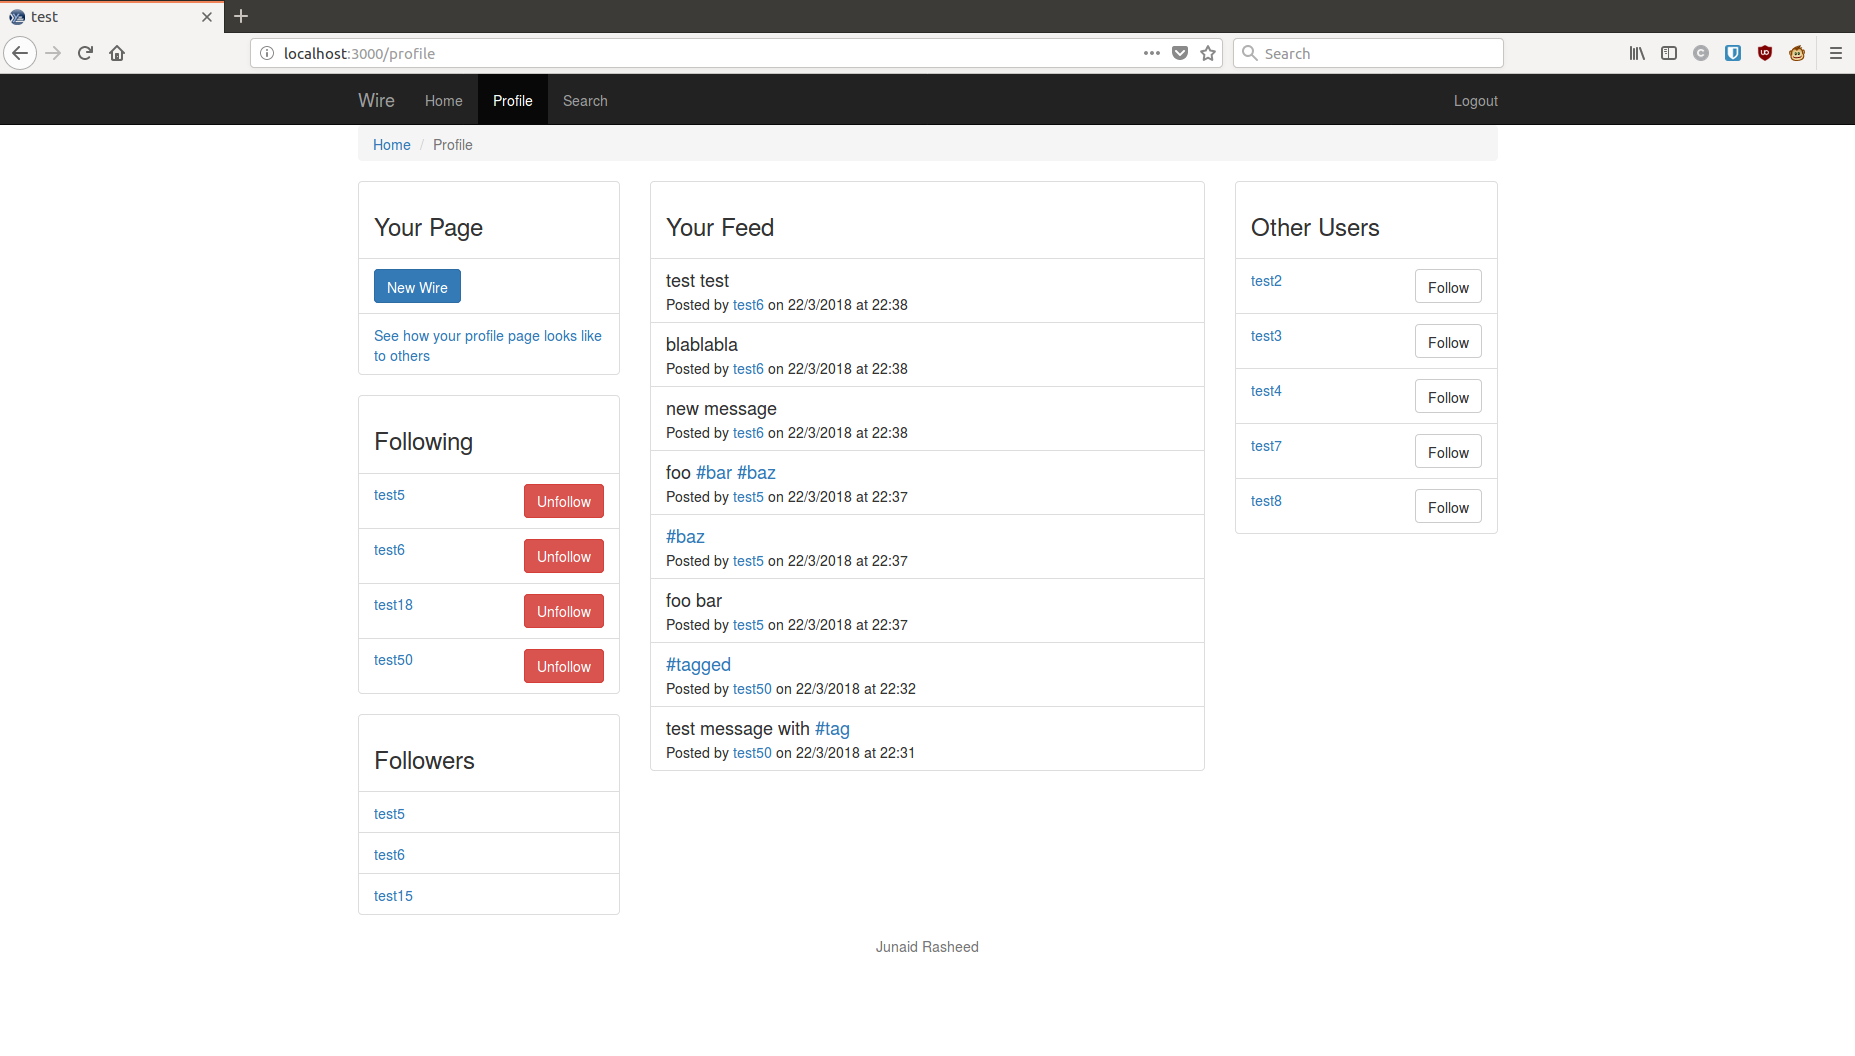
\includegraphics[width=0.7\textwidth]{final_report/pics/profile.png}
	\caption{The profile page for the current user}
	\label{fig:wireProfile}
\end{figure}

\begin{figure}[H]
	\centering
	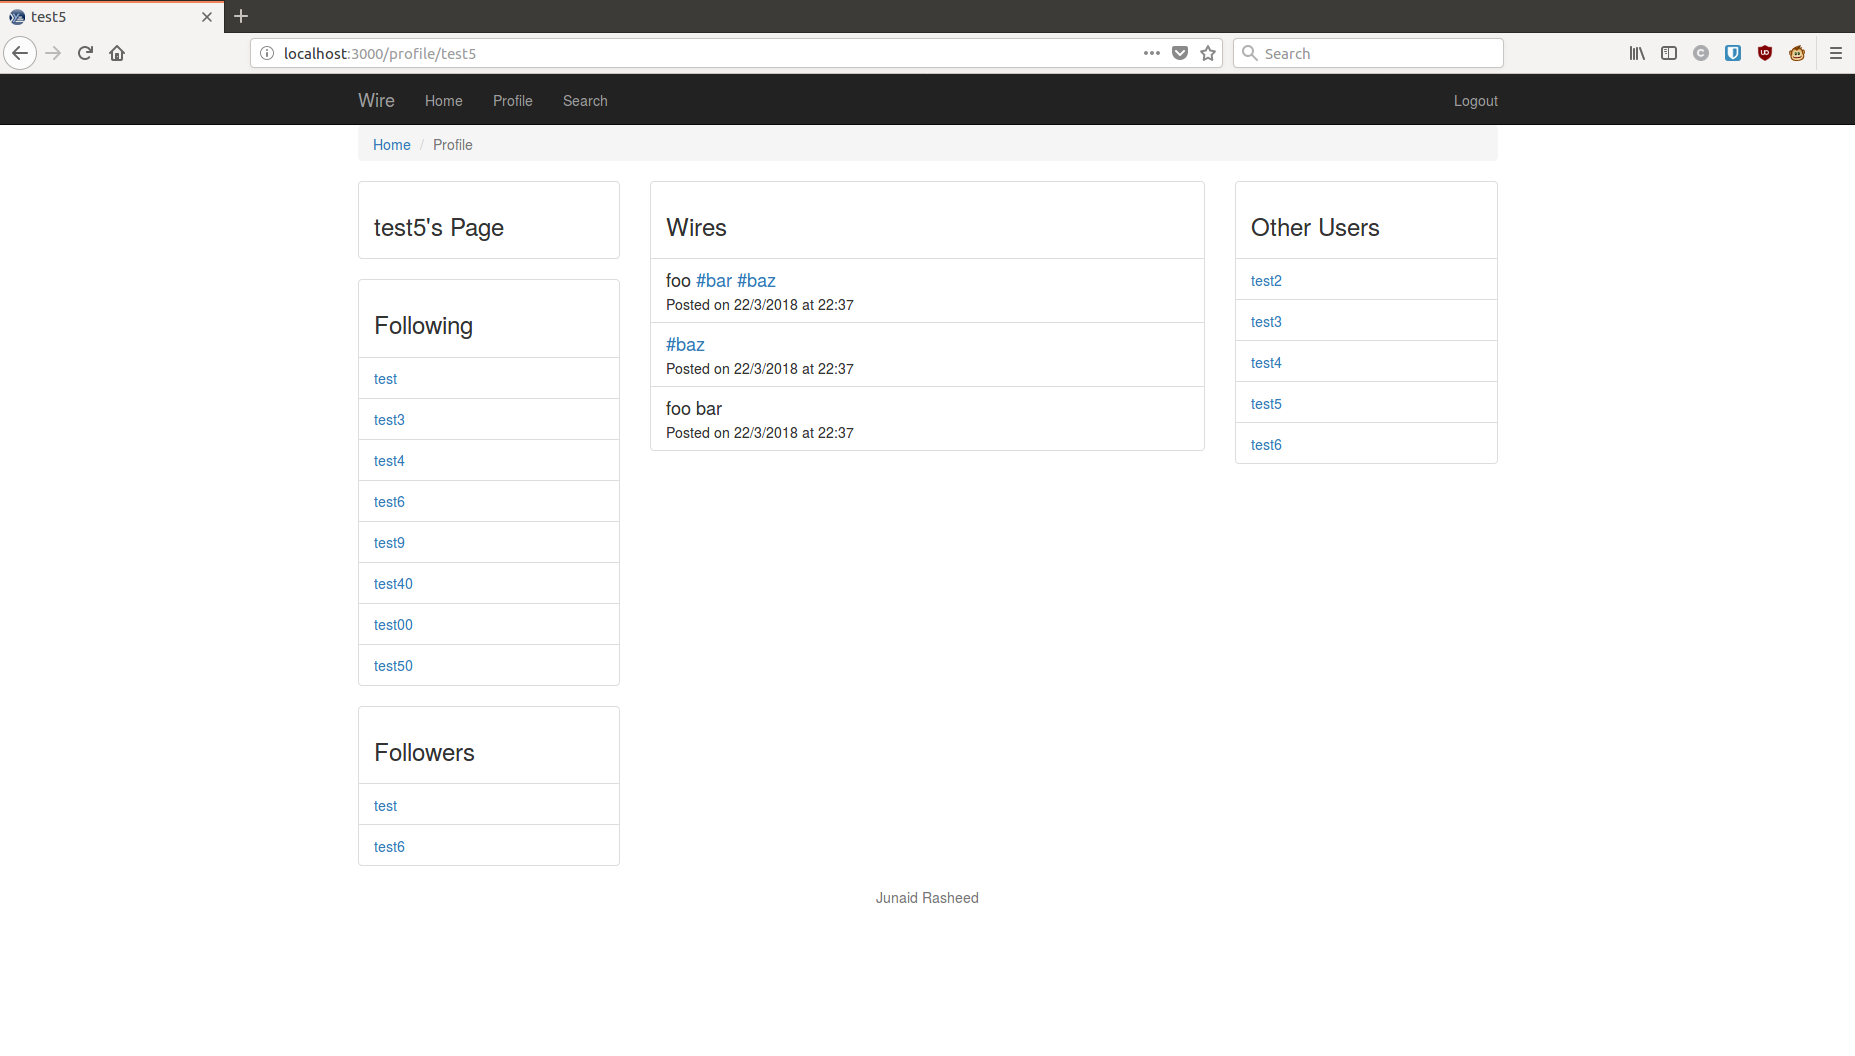
\includegraphics[width=0.7\textwidth]{final_report/pics/otherProfile.png}
	\caption{The profile page for other users}
	\label{fig:wireOtherProfile}
\end{figure}

\begin{figure}[H]
	\centering
	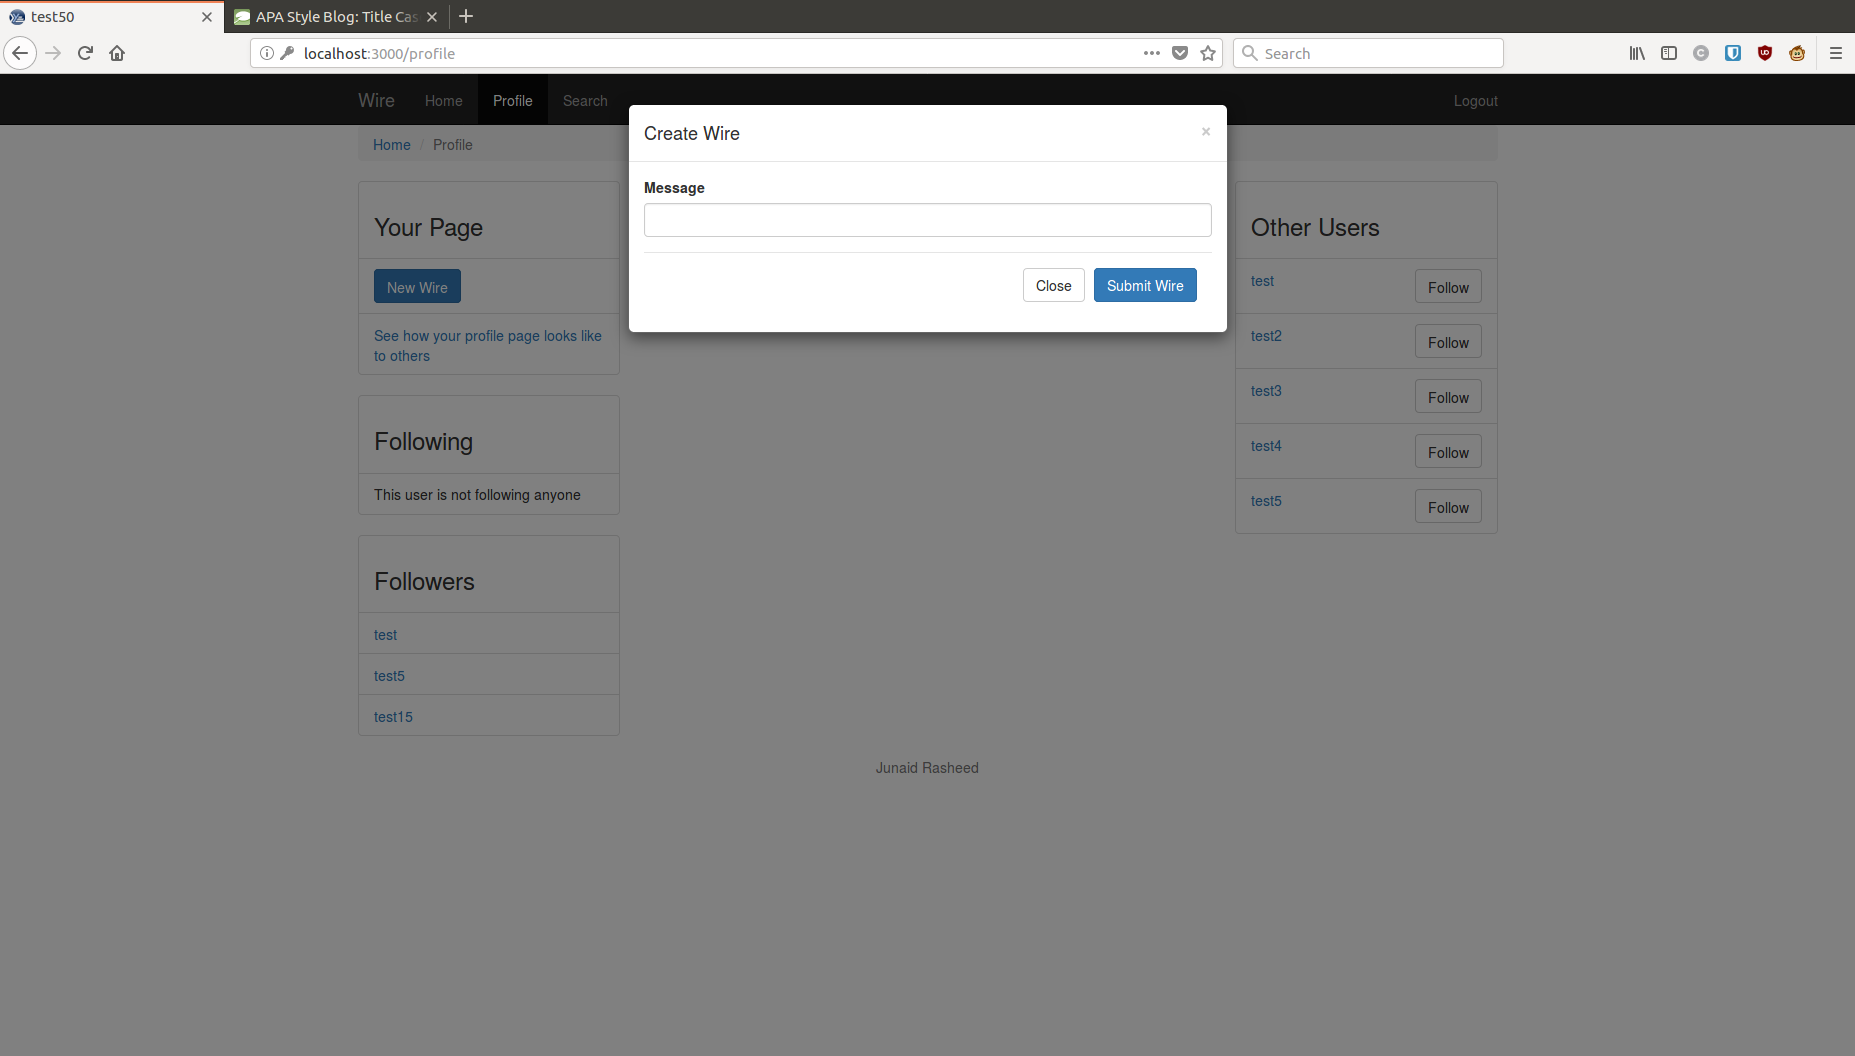
\includegraphics[width=0.7\textwidth]{final_report/pics/createWireForm.png}
	\caption{The create message form}
	\label{fig:wireCreateForm}
\end{figure}


The profile pages are probably the most complex with regards to logic in the
entire website. There are two different profile pages, one for the currently
logged in user which only they can see, and another for when someone is
viewing the profile page of another user.

Figure ~\ref{fig:wireProfile} is what a logged in user sees if they visit
their own profile page. On this page, they can see a list of messages posted
by users that they follow, see which users are following them, follow and
unfollow other users, and post their own messages. They can also post a
new message by clicking on the `New Wire' button. Clicking this button
displays a form which can be seen in figure ~\ref{fig:wireCreateForm}.

Figure ~\ref{fig:wireOtherProfile} is what the profile page looks like
when a user navigates to another person's profile page, or when they click
the `See how your profile page looks like to others' link on their own
profile page. This page shows the name of the person who owns the page,
the users they follow, other users that follow them, and messages that
they have posted.

One feature to note is that the messages and other user information on
the profile page is loaded in via AJAX. This ensures that the initial
page load is quick, following and unfollowing users does not necessitate
an entire page reload, and makes it easier to, if desired, add a feature
to automatically update the message area.

\subsection{The Search Page}

\begin{figure}[H]
	\centering
	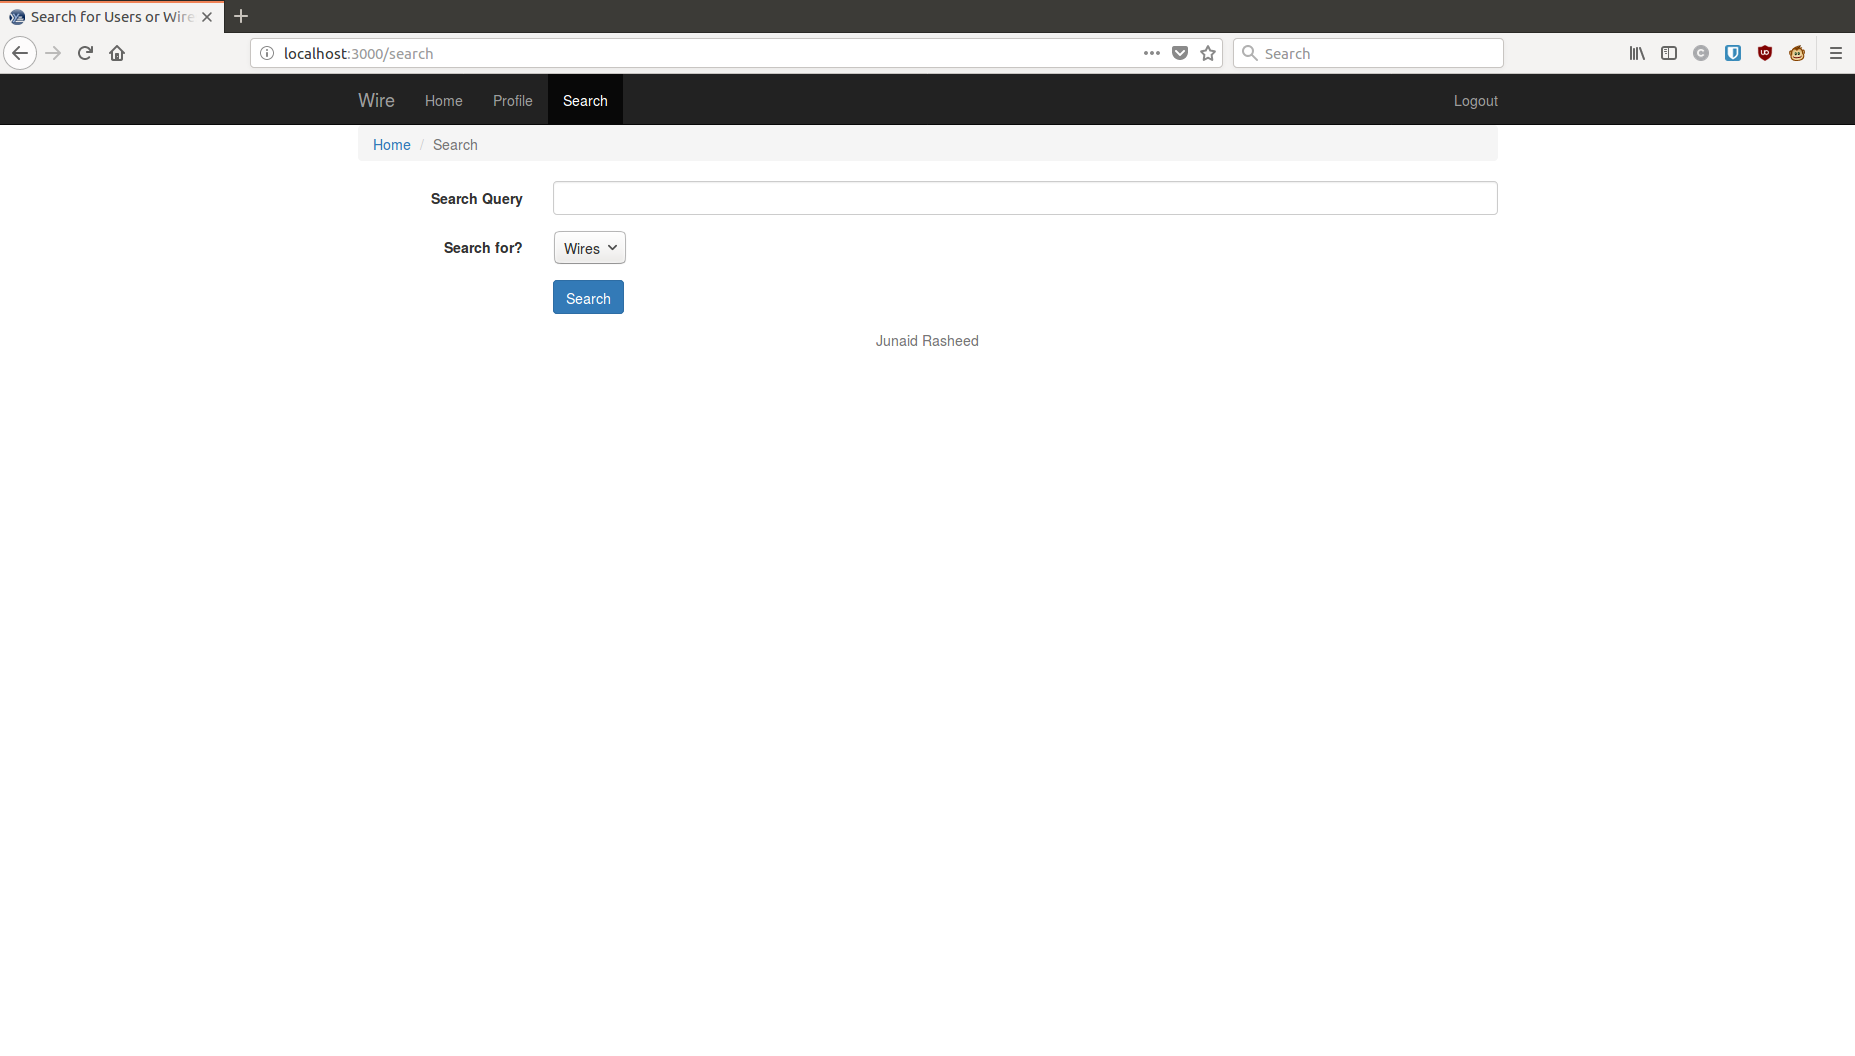
\includegraphics[width=0.7\textwidth]{final_report/pics/searchBase.png}
	\caption{The search page}
	\label{fig:wireSearch}
\end{figure}

\begin{figure}[H]
	\centering
	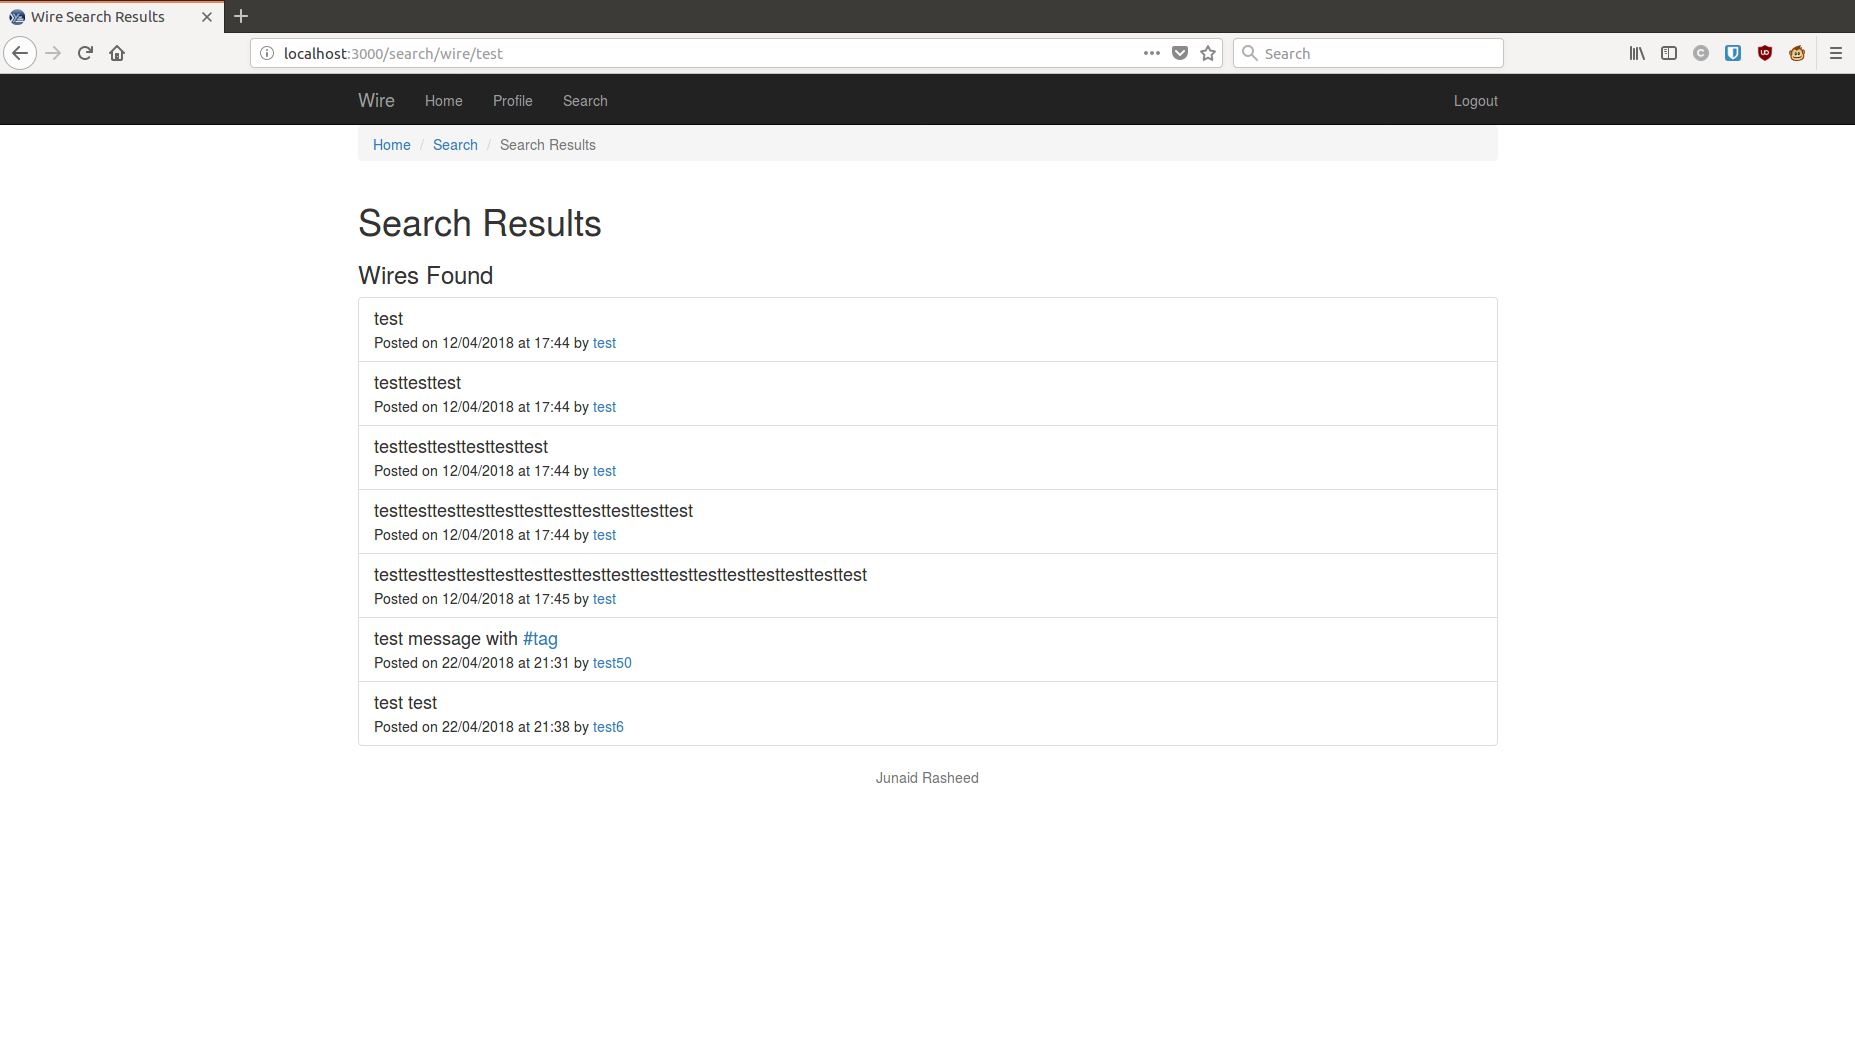
\includegraphics[width=0.7\textwidth]{final_report/pics/searchWire.png}
	\caption{The search results page for messages}
	\label{fig:wireSearchWire}
\end{figure}

\begin{figure}[H]
	\centering
	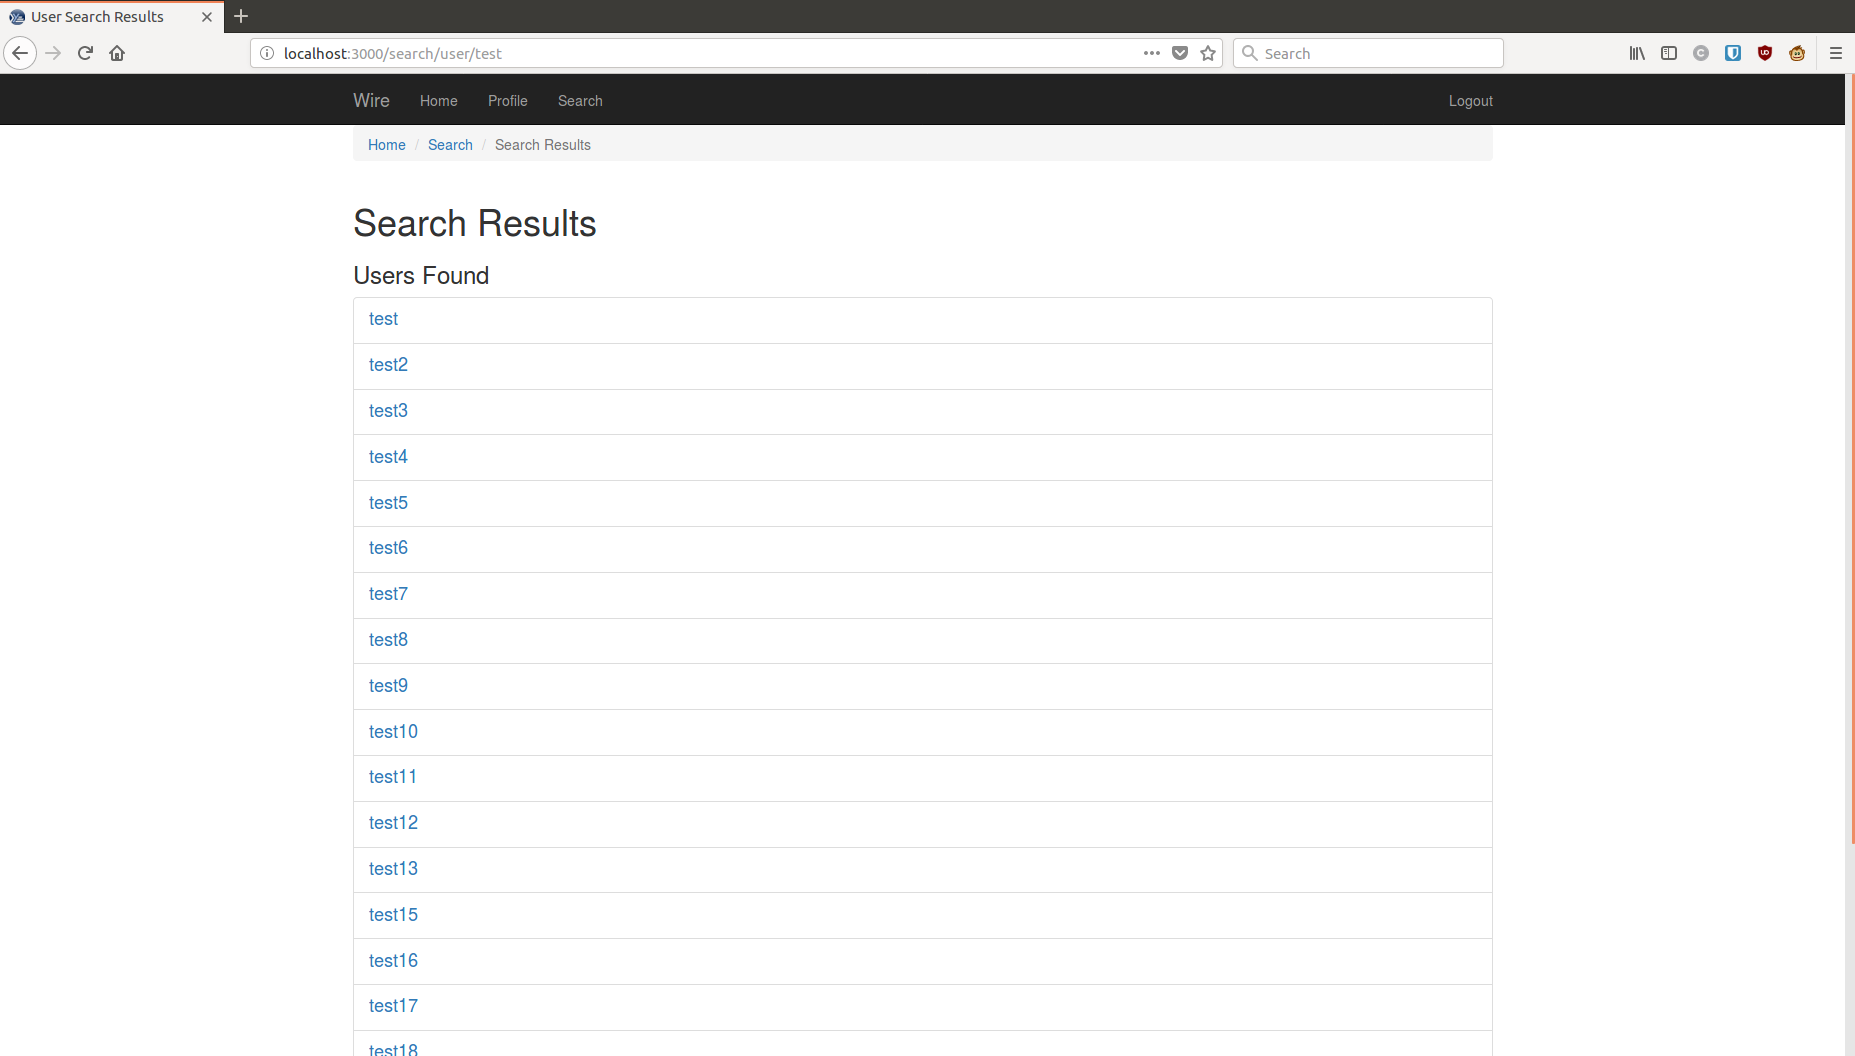
\includegraphics[width=0.7\textwidth]{final_report/pics/searchUser.png}
	\caption{The search results page for other users}
	\label{fig:wireSearchUser}
\end{figure}

Figure ~\ref{fig:wireSearch} is the page that the user is navigated to when they
click the search button in the navigation bar. In this page, they can type in
their search query and use the dropdown to specify whether they are searching
for users or messages. Once they submit their query, they are redirected to
the search results page, as seen in Figures ~\ref{fig:wireSearchUser} and
~\ref{fig:wireSearchWire}.

\section{The Yesod Implementation}

In this section, we will briefly discuss how the website was implemented in Yesod.
We will take a look at creating database entities, URL routing, handling requests,
creating templates, and writing tests.

\subsection{The Scaffold}
When creating a new Yesod site, it is recommended to use the scaffolding tool.
The scaffolding tool generates code that sets up the structure of your project. It
creates the files needed to connect to a database and launch a website. Sample code
is included for developers to see how the framework works. By running the scaffolding
tool, it is clear to the developer where source files, configuration settings, templates, and 
static files should be kept. \parencite[Scaffolding and the Site Template]{yesodBook}

The Yesod codebase used for this project was built on top of code generated by the
scaffolding tool using the yesod-postgres template, which tells the generated code
to be compatible with a PostgreSQL database.

\subsection{Defining Routes}

URL routes are available routes in an application and are specified in the 
`config/routes' file. In this file, you specify whether a request from a route is a
GET or POST request, the handler that deals with the request, and any parameters
that are part of the request. One of the features of Yesod is type safety in URLs,
so you can specify the actual type that a URL parameter should be. If the user
tries to navigate to a page with an invalid parameter, a 404 page will be shown.
An extract from the `config/routes' file can be seen in code block 
~\ref{code:yesodRoutes} below.

\lstset{language={}}

\begin{lstlisting}[caption={Yesod URL routes},label={code:yesodRoutes}]
	/profile MyProfileR GET POST
	/profile/#Text ProfileR GET
	
	/user UserGetAllR GET
	/user-not-following UserGetAllExcludingFollowingR GET
	/user/#Text UserGetAllExcludingUsernameR GET
	/user/id/#UserId UserGetIdR GET
	/users/*[UserId] UserGetIdsR GET
\end{lstlisting}

In code block ~\ref{code:yesodRoutes}, you can see that there
are two routes for the profile page. One, \texttt{/profile}, is for users
viewing their own profile page and the other, \texttt{/profile/\#Text}, are
for viewing the profile pages of the other users. The \texttt{\#Text} part
of the route specifies that there should be one parameter for this
route with the type \texttt{Text}. If multiple parameters are provided or a parameter
is not of the type \texttt{Text}, a 404 error is shown.

Further examples of URL parameters can be seen in the \texttt{user} routes. 
\texttt{/user/id/\#UserId} expects a user id as a parameter. If the specified
id is not found, a 404 page is shown. \texttt{/users/\*[UserId]} expects a list
of user ids, which would look like \texttt{/users/1/2/3/4/}.

\subsection{Database Entities}

Database entities are defined in the `config/model' file. In this file, you
give a name to the entity you want to create, the names and types of it's
fields, functions that the entity and it's fields should include, and
any fields that are unique, i.e. Cannot be shared with other entities.
Once an entity is added to this file, it is created in the database
when the codebase is compiled and helper functions are created that
can be used when programming. Code block ~\ref{code:yesodEntities} contains
the definition of the user entity extracted from the `config/models' file.

\begin{lstlisting}[caption={Yesod Database Entities},label={code:yesodEntities}]
	User json key
		username Text Eq
		email    Text Eq
		password Text
		UniqueUser username
		UniqueEmail email
		deriving Typeable Show
\end{lstlisting}

\subsection{Handlers}

Every URL route in the application points to a handler. Handlers are located in
the \texttt{src/handler} directory. They are used to perform any calculations or queries 
that need to be done and then respond to a request by rendering a template file, 
returning a JSON object, or by redirecting to another handler.

Code block ~\ref{code:yesodGetProfileR} is the handler used to respond to get requests
to display the profile page of the current user. The handler ensures the user is logged in,
loads the user's details, loads data on people being followed by the current user,
and then loads the template file. The parameters that are created and available
in the handler are also available in the template file.

\lstset{language={Haskell}}

\begin{lstlisting}[caption={GET request handler for current profile page},label={code:yesodGetProfileR}]
	-- Loads the 'My Profile' page for the currently logged in user. If someone
	-- who is not logged in attempts to access the page, a 404 error will be shown.
	getMyProfileR :: Handler Html
	getMyProfileR = do
		(Entity userId user) <- requireAuth
		let username = userUsername user
	
		-- Load messages posted by users followed by the current user
		follows <- runDB $ selectList [FollowFollowingId ==. userId] []
		let followIds = map (\(Entity _ (Follow followerId _)) -> followerId) follows
	
		(formWidget, formEnctype) <- generateFormPost $ messageForm userId
		defaultLayout $ do
			setTitle . toHtml $ userUsername user
			$(widgetFile "currentprofile")
\end{lstlisting}

You may have noticed the message form being generated in code block ~\ref{code:yesodGetProfileR}.
This form is defined in Haskell and the source code can be seen in code block ~\ref{code:yesodMessageForm}.
When defining the form, we give it a user id to specify the user creating a message, 
we tell the form that there is one input field that is required. Two hidden fields
are also included to ensure the form has all the data needed to create a message
when it is submitted.

\begin{lstlisting}[caption={The message form},label={code:yesodMessageForm}]
	messageForm :: UserId -> Form Message
	messageForm userId = renderBootstrap3 BootstrapBasicForm $ Message
		<$> areq textField (bfs ("Message" :: Text)) Nothing
		<*> pure userId
		<*> lift (liftIO getCurrentTime)
\end{lstlisting}

When the user submits the form, the post handler is ran, which can be seen in code block
~\ref{code:yesodPostProfileR}. In this handler, we use the function \texttt{runFormPost}
to check whether or not the form is valid. If the form is valid, the message is added
to the database and the profile page is reloaded with a success message. If there's an
issue with the form, the profile page is reloaded with an appropriate error message.

\begin{lstlisting}[caption={POST request handler for current profile page},label={code:yesodPostProfileR}]
	-- Create a new wire for the logged in user
	postMyProfileR :: Handler Html
	postMyProfileR = do
		(Entity userId _) <- requireAuth
		((result, _), _) <- runFormPost $ messageForm userId
		case result of
			FormSuccess message -> do
				void $ runDB . insert $ message
				setSession "msgrendered" "true"
				setMessage $ renderSuccessMessage "Wire Sent"
				redirect MyProfileR
			FormFailure errors -> do
				let renderedMessages = map renderErrorMessage errors
				setSession "msgrendered" "true"
				setMessage $ toHtml renderedMessages
				redirect MyProfileR
			FormMissing -> do
				setSession "msgrendered" "true"
				setMessage $ renderErrorMessage "Form is missing"
				redirect MyProfileR
\end{lstlisting}

If a route contains a URL parameter, the handler must also have a parameter to store
the value of the given parameter. Code block ~\ref{code:yesodGetUserGetIdR} is the
source code for a handler that takes in a user id as a parameter. As you can see,
we do not have to check for the type of this parameter or whether it is not null.
We specified the type of the URL parameter in the routes file (code block ~\ref{code:yesodRoutes})
so Yesod will perform type checking for us, saving developers time from having
to manually deal with invalid types or values.

\begin{lstlisting}[caption={GET request handler for getting user data},label={code:yesodGetUserGetIdR}]
	-- | Takes in a user id and returns data on the user matching the given id.
	-- If no user is found, an empty JSON object is returned.
	getUserGetIdR :: UserId -> Handler Value
	getUserGetIdR userId = do
		users <- runDB $ selectList [UserId ==. userId] []
		let cleanUsers = map (\(Entity uid (User uname _ _)) -> (object ["id" .= uid, "username" .= uname])) users
		returnJson cleanUsers
\end{lstlisting}

\subsection{Templates}

The templates used in Yesod are called Shakespearean templates. Shakespearean templates
allow you to write type-safe templates that are compiled, helping prevent runtime errors.
The syntax for Shakespearean templates are similar to the languages they are based on,
with minor changes to the syntax used in the templates. For example, the HTML template language, Hamlet,
uses indentation rather than opening and closing tags to denote nesting. Within these
templates, you can use Haskell variables, create type-safe routes, and implement conditional
and looping logic. \parencite[Shakespearean Templates]{yesodBook}

When a template file is loaded in a handler, the file is actually included inside
a default file. The default file contains content that is common to all pages. This
ensures that code does not need to be repeated, reducing the chance of mistakes and
making it easier to change the layout of the whole site.

A simple template file can be seen in code block ~\ref{code:yesodSearchHamlet}. In this
block, you can see how indentation is used to determine nesting. Variable interpolation
is done using \texttt{\#\{variableName\}}. You can see the form is being loaded using
the \texttt{\string^\{widgetName\}}, which renders the given widget onto the page. Type safe
URLs are loaded using \texttt{\string@\{routeName optionalParameters\}}.

\begin{lstlisting}[caption={Template file for the search page},label={code:yesodSearchHamlet}]
	<main>
		<div .container>
			<div .row>
				<div .col-sm-12>
					<form #search-form .inline .form-horizontal role=form method=post action=@{SearchR} enctype=#{formEnctype}>
						^{formWidget}

\end{lstlisting}

\subsection{Tests}
The Yesod test suite allows you to create BDD-style tests. When creating a test,
you specify what it should do, create any database entities you need, make a
request to a handler, and examine the response to see if the data you received
is correct. Code block ~\ref{code:yesodGetProfileTest} is an actual test
from the website. The test creates and logs in as a new user, loads
the profile page, and ensures that the resulting HTML contains the text that
it should contain. Yesod gives you the ability to use CSS selectors when checking
the HTML page given by a response, allowing you to be very specific.

\begin{lstlisting}[caption={Test the profile page},label={code:yesodGetProfileTest}]
	it "asserts that the current profile page looks right" $ do
		foo <- createUser "foo" "foo@bar.com" "foo"
		authenticateAs foo

		get MyProfileR
		htmlAnyContain "h3" "Your Page"
		htmlAnyContain "h3" "Your Feed"
		htmlAnyContain "h3" "Followers"
		htmlAnyContain "h3" "Following"
		htmlAnyContain "h3" "Other Users"
\end{lstlisting}

The testing suite also has the ability to check if a JSON response contains the
data that we expect. However, you do not have the same helper functions available
to you when compared to checking HTML responses. When checking JSON response, you
must examine the body of the response itself. You cannot check if a JSON key has
a given value. See code block ~\ref{code:yesodGetAllUsers} below.

\begin{lstlisting}[caption={Checking a JSON response},label={code:yesodGetAllUsers}]
	it "asserts all users are returned when not authenticated" $ do
		_ <- createUser "foo" "foo@bar.com" "foo"
		_ <- createUser "bar" "bar@bar.com" "foo"
		_ <- createUser "baz" "baz@bar.com" "foo"

		get UserGetAllR

		bodyContains "username"
		bodyContains "id"
		bodyNotContains "email"
		bodyNotContains "password"
		bodyContains "foo"
		bodyContains "bar"
		bodyContains "baz"
\end{lstlisting}
\section{The Django Implementation}
Now, we will discuss how the Django site was implemented. We will go through Django apps,
routes, entities, views, templates, and tests.

\subsection{Creating a Project}
All Django sites require a Django project. A project is
a directory that contains all the settings needed for a Django website. This includes
database settings, the apps being used, application settings, and Django-specific
settings. To create the project, the \texttt{django-admin} tool was used. This tool
generates the code needed to connect to a database and start a Django site. \parencite{djangoIntroDocs}

\subsection{Creating Apps}

The code used for the actual web application resides in two Django apps, \texttt{base} and
\texttt{wire\_profile}. In Django, an app is a web application that can be a part of a project.
These apps contain the URL routes used in the application, database entities, views
that respond to requests, templates, and tests. The \texttt{manage.py} tool provided
by Django was used to create apps. This tool creates a directory with a specified name
and a layout of files and directories that is preferred for Django apps. \parencite{djangoIntroDocs}

\subsection{Routes}

Django routes are specified in the \texttt{urls.py} file within an app. The routes
specify a URL path, a view that responds to requests from the given path, and a name
that is used to refer to a route within code. Django routes can contain URL parameters,
like Yesod. The valid values for these parameters can be defined using regular expressions
or a few built in types like \texttt{string} or \texttt{int}. To denote a list of parameters,
\texttt{path} can be used. An example of Django routes can be seen in code block ~\ref{code:djangoRoutes}.

\lstset{language={Python}}

\begin{lstlisting}[caption={An extract of Django routes},label={code:djangoRoutes}]
	path('following/<path:username>', views.get_following, name='get_following'),
	path('users/<path:user_ids>', views.get_user_ids, name='get_user_ids'),
	path('user/id/<int:user_id>', views.get_user_id, name='get_user_id'),
	path('search', SearchView.as_view(), name='search'),
\end{lstlisting}

\subsection{Database Entities}

Database entities are defined as models in the \texttt{models.py} file within an app.
In this file, the name of a database entity is mapped to a class in the file. The variables inside
this class are used to determine the names and types of entity's fields. You can see
an example of a Django model in ~\ref{code:djangoEntities}. When an entity is created 
or modified, Django migrations must be created and then ran using the \texttt{manage.py} tool. 
Migrations are used by Django to ensure changes you make to models are executed in 
the database schema. \parencite{djangoMigrations}.

\begin{lstlisting}[caption={The user entity in Django},label={code:djangoEntities}]
	class Message(models.Model):
	message_text = models.CharField(max_length=280)
	created = models.DateTimeField('created')
	user = models.ForeignKey(User, on_delete=models.CASCADE)

	def __str__(self):
		return self.message_text
\end{lstlisting}

\subsection{Views}

Views in Django are similar to Handlers in Yesod, they are used to determine
a response for a given request. There are two main types of views that you can
create in Django, class-based views and function-based views. The Django website
produced contains a mixture of class-based and function-based views.

Code block ~\ref{code:djangoCurrentProfileView} is a class-based view used to
render the profile page for the current user. In this view, we check if the
user is authenticated and then render the profile page for the authenticated
user. If the user is not authenticated, we redirect them to the home page and
show an error message.

\begin{lstlisting}[caption={Class-based current profile view},label={code:djangoCurrentProfileView}]
	class CurrentProfileView(TemplateView):
	template_name = "wire_profile/current_profile.html"

	def get(self, request, *args, **kwargs):
		"""
		Get the current profile if the user is logged in.

		:param request: The current request
		:param args: sent to parent method
		:param kwargs: sent to parent method
		:return: Either redirect to the search page or render the profile page
		"""
		if request.user.is_authenticated:
			context = self.get_context_data(**kwargs)
			form = NewWireForm()
			context['form'] = form
			context['user'] = request.user
			return self.render_to_response(context)
		else:
			messages.error(request, 'You must log in to view your profile page', extra_tags='danger')
			return HttpResponseRedirect(reverse('base:home'))
\end{lstlisting}

In the current profile view, we load a Django form for a user to create a message,
just like we do in Yesod. This form is located in the \texttt{forms.py} file. The
form, as seen in code block ~\ref{code:djangoMessageForm}, is a class where variables map
to input names. The Django form only requires one field, the message. No hidden
fields are used to determine the user that created a message, this is done in
the view itself.

\begin{lstlisting}[caption={Django message form},label={code:djangoMessageForm}]
	class NewWireForm(forms.Form):
		message = forms.CharField(widget=forms.Textarea(attrs={'rows': '3', 'cols': '40'}), label='Message', max_length=280)
\end{lstlisting}

When the form is submitted, a post request is sent to the function-based view
seen in code block ~\ref{code:djangoCreateMessageView}. In this view, the following
conditions are checked: whether or not the request type is POST, the validity of the
form, and whether or not the user is authenticated. If these conditions are true,
the message is created and saved to the database. If not, an appropriate error
message is rendered.

\begin{lstlisting}[caption={Function-based create message view},label={code:djangoCreateMessageView}]
	def create_message(request):
		"""
		Create a message for the logged in user

		:param request: The request sent by the user
		:return: Display the profile page with a relevant message
		"""
		if request.method == 'POST':
			form = NewWireForm(request.POST)
			if form.is_valid():
				if request.user.is_authenticated:
					message = form.cleaned_data['message']
					try:
						Message.objects.create(message_text=message, created=timezone.now(), user=request.user)
						messages.success(request, 'Message created successfully', extra_tags='success')
						return HttpResponseRedirect(reverse('wire_profile:current_profile'))
					except DatabaseError:
						messages.error(request, 'Error creating message, please contact support', extra_tags='danger')
						return HttpResponseRedirect(reverse('wire_profile:current_profile'))
				# ... each else condition renders an appropriate error message
\end{lstlisting}

The method to retrieve URL parameters in Django differ depending on the type
of view you use. For class-based views, URL parameter values are retrieved using
the \texttt{kwargs} variable available in all class-based views, as seen in
code block ~\ref{code:djangoSearchMessage}. For function-based views, a
parameter is added to the function itself, as seen in code block ~\ref{code:djangoGetUserIds}. 

\begin{lstlisting}[caption={Function-based view for returning user data},label={code:djangoGetUserIds}]
	def get_user_ids(request, user_ids):
		"""
		Get the users with the given IDs in JSON format

		:param request: The request that called this function
		:param user_ids: The user ids to get the users for
		:return: list of users in JSON format
		"""
		user_ids_list = filter(bool, user_ids.split('/'))
		user_ids_list = list(map(int, user_ids_list))
		% users = User.objects.filter(pk__in=user_ids_list).values('username')
		return JsonResponse(list(users), safe=False)
\end{lstlisting}

\begin{lstlisting}[caption={Class-based view to search for a given message},label={code:djangoSearchMessage}]
	class SearchMessageView(TemplateView):
		template_name = 'wire_profile/search_message.html'

		def get(self, request, *args, **kwargs):
			"""
			Render the matching messages for a search message query

			:param request: The current request
			:param args: sent to parent method
			:param kwargs: sent to parent method
			:return: Render the search message results page
			"""
			query = self.kwargs['query']
			search_results = Message.objects.filter(message_text__icontains=query).all()
			context = self.get_context_data(**kwargs)
			context['search_results'] = search_results
			return self.render_to_response(context)
\end{lstlisting}

\subsection{Templates}
The Django template language can be used in any HTML, CSS, and JavaScript
file. The Django template language can be used to perform variable interpolation,
conditional checks, loops, and creating default blocks of code that can be reused
in other templates. Rendering these files executes the the template logic that the
file contains. \parencite{djangoTemplates}

\begin{lstlisting}[caption={Template file for the search page},label={code:djangoSearchTemplate}]
	

	
	
	
	
	
		{{ block.super }}
		
	
	
	
		Search
	
	
	
	<main>
		<div class="container">
			<div class="row">
				<div class="col-sm-12">
					<form id="search-form" class="inline form-horizontal" role=form method=post action="/search">
						
						
					</form>
				</div>
			</div>
		</div>
	</main>
	
\end{lstlisting}

Code block ~\ref{code:djangoSearchTemplate} contains the source code for the
template file used to render the search page. In this file, a base template
is loaded, which is a full HTML page with the content divided up
into a number of blocks. These blocks are then overridden in the search template
to define breadcrumbs, set the page title, and write the markup for the main
content of the page. Laying out template files like this eliminates repetitive
code and keeps the Django template files similar to their Yesod counterparts,
reducing the need to design different templates in both frameworks.

\subsection{Tests}

Django tests are contained in the \texttt{tests.py} file within an app. Tests
are functions within a class. The process for testing in Django is similar to
Yesod: we create any needed database entities at the beginning of a test,
make a request, and check to see if the response is what we expect. Code
block ~\ref{code:djangoCurrentProfileTest} is a test where a user account
is created, logged in, and then the profile page for the user is loaded.
Django does not have the functionality available in Yesod that allows you
to test the content of a HTML page using CSS selectors, so instead, we test
that the correct template is being loaded with the expected template variables.

\begin{lstlisting}[caption={Django current profile test},label={code:djangoCurrentProfileTest}]
	class CurrentProfileViewTest(TestCase):
		# Other tests...
		def test_current_profile_page_for_logged_in_users(self):
			user = User.objects.create_user('testfoo', 'test@test.com', 'test')
			self.client.post(reverse('base:verify'), {'username': user.username, 'password': 'test'})
			response = self.client.get(reverse('wire_profile:current_profile'))

			self.assertEqual(response.status_code, 200)
			self.assertEqual(response.context['user'], user)
			self.assertIsInstance(response.context['form'], NewWireForm)
			self.assertTemplateUsed(response, 'wire_profile/current_profile.html')
\end{lstlisting}

In Django, we can still examine the content of a response, as seen in code block ~\ref{code:djangoCheckJsonResponse}.
In this block, we make a JSON request decode the response, ensuring that the response
content contains the expected data.

\begin{lstlisting}[caption={Django checking a JSON response test},label={code:djangoCheckJsonResponse}]
	class GetUserIdsTest(TestCase):
		# Other tests...
		def test_get_user_ids_one_user(self):
			user = User.objects.create_user('foo', 'test@test.com', 'test')
			user2 = User.objects.create_user('bar', 'bar@test.com', 'test')
			user3 = User.objects.create_user('baz', 'baz@test.com', 'test')

			response = self.client.get(reverse('wire_profile:get_user_ids', kwargs={'user_ids': str(user.id) + '/'}))
			response_content = response.content.decode()

			self.assertEqual(response.status_code, 200)
			self.assertIn('"username": "' + user.username + '"', response_content)
			self.assertNotIn('"username": "' + user2.username + '"', response_content)
			self.assertNotIn('"username": "' + user3.username + '"', response_content)
\end{lstlisting}

\section{Comparison of Django and Yesod}

This section consists of a comparison of both frameworks. A series of experiments
were conducted as specified in the plan, the raw results of which can be found
in appendix ~\ref{app:Experiments}. These results will be discussed along with
features and limitations of both frameworks that stand out.

To ensure that the results we collected were as fair as possible, two Amazon
EC2 servers were created. The configuration of both servers were identical,
with them having 1GB of RAM and 1 CPU core available. The tools necessary
to deploy the website were installed on both servers and both sites were
released on the server, allowing testing to begin.

\subsection{Deployment}

Deploying a Yesod onto an Amazon EC2 app is very simple. Yesod has built-in
support for a tool called Keter, a Haskell application that can act as a
web server. After Keter was installed and configured on the Amazon EC2 server,
a Keter binary was created using commands built-in to Yesod. This binary
file can simply be transferred onto the server, and Keter will start serving
the web application to visitors. \parencite[Deploying your Webapp]{yesodBook}

For the Django website, nginx, an open source web server was installed. nginx
acts as a reverse proxy to the Django application, which is being run by a tool
called Gunicorn (`Green Unicorn'). Gunicorn is a WSGI (`Web Server Gateway
Interface') tool that can be used on Unix systems. \parencite{djangoGunicorn} This means that Gunicorn
can allow nginx to use Django to serve the web application.

\subsection{Page Load Speed}
\label{sec:pageLoadSpeed}

When testing page load speeds, each page was loaded three times. The time
taken for each run was recorded as well as an average. In this section,
we will be discussing the average times that were recorded. The raw
results can be found in section ~\ref{sec:pageLoadSpeeds} in the appendix.

Page load speeds for Yesod are noticeably quicker than Django, with Yesod
loading most pages around 200ms faster. For example, on average, the home page
takes about 511ms to load in the Yesod framework, and 750ms to load in the
Django framework. Creating a new message and then redirecting back to the
profile page takes about 679ms in Yesod and 849ms in Django. See
table ~\ref{tab:pageLoadAverageSpeeds} for a full list of results.

\begin{table}[H]
	\caption{Average Page Load Speeds}
	\begin{center}
		\begin{tabular}{ | l | r | r |}
			\hline
			Page & Average Speed in Yesod (ms) & Average Speed in Django (ms) \\
			\hline
			Home Page & 511.00 & 753.33 \\
			Search Page & 517.33 & 756.33 \\
			Login Page & 443.67 & 821.33 \\
			Signup Page & 490.33 & 764.00 \\
			Creating an Account & 504.33 & 748.67 \\
			Logging in to an Account & 547.33 & 722.67 \\
			Logging out & 510.33 & 761.33 \\
			Current user's Profile Page & 617.00 & 930.00 \\
			Other user's Profile Page & 651.33 & 908.67 \\
			Creating a Message & 679.33 & 848.67 \\
			Search for a Message & 513.33 & 766.33 \\
			Search for a User & 519.00 & 756.67 \\
			\hline
		\end{tabular}
	\end{center}
	\label{tab:pageLoadAverageSpeeds}
\end{table}

As you can see in table in table ~\ref{tab:pageLoadAverageSpeeds}, Yesod
consistently outperforms Django. This could be for a number of reasons:
Yesod automatically minimises static files like CSS or JavaScript;
Haskell is compiled rather than interpreted, and compiled code generally
runs faster than interpreted code; the lazy evaluation of Haskell may
give some speed improvements; and the Keter tool used on the server
is made specifically for Haskell web applications, which may mean that
Yesod and Keter will run faster than Django and nginx.

\subsection{Load Tests}

Load tests were conducting using a tool called RedLine13. RedLine13 is
a service that allows users to perform load testing using Amazon EC2
servers. With RedLine13, I was able to send requests from an Amazon
EC2 server to the Yesod and Django websites. To keep within the
usage limits of RedLine13 and Amazon EC2, three load tests were
conducted. Each test had 80 users load a specific page in a short
amount of time, typically 25 seconds. The results of these tests can
be found in table ~\ref{tab:loadTests}.

\begin{table}[H]
	\caption{Load Testing Page Load Speeds}
	\begin{center}
		\begin{tabular}{ | l | l | l |}
			\hline
			Page & Yesod (s) & Django (s) \\
			\hline
			Home & 4.96 & 5.54 \\
			Profile & 5.05 & 4.94 \\
			Profile & 4.97 & 5.13 \\
			Average & 4.99 & 5.20 \\
			\hline
		\end{tabular}
	\end{center}
	\label{tab:loadTests}
\end{table}

As you can see in the table above, Yesod is around 200ms faster than
Django when under load. This difference is consistent with the results
found in section ~\ref{sec:pageLoadSpeed}. The high loading times
seen in these tests is probably because the servers are being are not
very powerful.

The tests also recorded the total amount of data downloaded for all
users. Yesod beat Django by a sizeable margin in this test, with
Yesod sending, on average, 6.46MB of data per test and Yesod
sending 18.19MB of data. This could be because Yesod, by default, 
minimises static files before sending them over to the client.

\subsection{Resource Usage}

Resource usage on both servers was measured after running the experiments
detailed in the section ~\ref{sec:pageLoadSpeed}. All the information in 
this section was obtained by examining output from htop, a process viewer. 
On the server running Yesod, 109MB of RAM was being used. The server running 
Django used 125MB of RAM.

To run a web server on the Yesod server, Keter creates two sub-processes.
One of these sub-processes loads the compiled code for the website, and the
other loads the configuration file for the web server. Altogether, these
three processes use about 83MB of RAM in total, with 56MB of RAM being
shared.

On the Django server, gunicorn, when run with the default settings, creates
one sub-process. These two processes use around 65MB of RAM and share 19MB
of RAM. nginx is not very memory intensive, using 6MB of RAM, sharing 3MB.
In total, the Django server uses 71M of RAM, sharing 22MB.

Yesod is ahead of Django when it comes to resource usage. Even though all the
Keter processes use more memory than gunicorn, most of the memory used by Keter
is shared, resulting in the overall memory usage in the Yesod server being lower
than the Django server. The RAM usage of the Django server is 16MB more than
the Yesod server, but this difference is Negligible considering the resources
available to most servers at this time.

\subsection{Continuous Integration}

For the duration of this project, all programming has been done on a git
repository stored on GitHub. Travis CI, a continuous integration tool,
syncs with GitHub in order to run tests on the repository every time
there is a new commit. The way this works is that every time a commit
is pushed to GitHub, GitHub sends the details of the commit to something
called a Webhook. Travis gets an update from this Webhook, and executes
a file called \texttt{.travis.yml} placed in the root of the repository.
This file contains instructions telling Travis how to run the tests
on the codebase.

Yesod did take longer to run tests when compared to Django. The Django
repository took around 2.5 minutes to build and run all the tests. Yesod
took around 3.5-4 minutes. For continuous integration, this difference
is negligible as any code will be peer reviewed in a real life before being
merged in to the main branch. For developing however, Django does speed
things along when you're implementing a new feature in a test driven way
and are running the test suite multiple times to ensure your feature
works and does not unintentionally break other features.

\subsection{Debugging}

When developing, you sometimes make mistakes. When you make these mistakes,
ideally, you would want to see an error message that tells you where you
made the mistake and some information about the error itself which may
help you resolve this mistake. As part of evaluating Yesod and Django,
simulated mistakes were made in both frameworks.

The first simulated mistake we made was, when creating a message, try
to save the form data object into the database rather than the actual
message stored inside this object. The code change in Yesod can be
seen in code block ~\ref{code:yesodMessageT1L}, and the Django change can
be seen in code block ~\ref{code:djangoMessageT1L}.


\lstset{language={Haskell}}
\begin{lstlisting}[caption={Yesod Code Change},label={code:yesodMessageT1L}]
	(Entity userId _) <- requireAuth -- get the user id
	((result, _), _) <- runFormPost $ messageForm userId -- get the form data
	case result of
		FormSuccess message -> do -- if it's a valid form, get the message
			-- _ <- runDB . insert $ message -- original line, insert message
			_ <- runDB . insert $ result -- new line, insert form data
\end{lstlisting}

\lstset{language={Python}}
\begin{lstlisting}[caption={Django Code Change},label={code:djangoMessageT1L}]
	form = NewWireForm(request.POST) -- get the form
	if form.is_valid():
		if request.user.is_authenticated:
			message = form.cleaned_data['message'] -- form.cleaned_data is a map of form values
			try:
				# Message.objects.create(message_text=message, ..) # original line, store the message
				Message.objects.create(message_text=form.cleaned_data, ..) # changed line 1, store form values
				# Message.objects.create(message_text=form, ..) # changed line 2, after previous line passed, store form object
\end{lstlisting}

For Yesod, the simulated error caused a compilation error, with the exception
message complaining about mismatched types, as seen in ~\ref{code:yesodT1E}. 
For Django, however, no exception was thrown, even when submitting the message. 
Further investigation showed that Python was converting the form data into a
string, and then saved this string in the database. Because the message was saved 
in the database, the tests, which at the time only checked the amount of objects
in the message table, passed. This test was later amended to check the actual
content of the message, and failed appropriately when the mistake was reintroduced.

\lstset{language={Haskell}}
\begin{lstlisting}[caption={Yesod Exception Message},label={code:yesodT1E}]
	- Couldn't match type `PersistEntityBackend (FormResult Message)'
	with `SqlBackend'
	arising from a use of `insert'
	- In the second argument of `(.)', namely `insert'
	In the expression: runDB . insert
	In a stmt of a 'do' block: _ <- runDB . insert $ result
\end{lstlisting}

In the second test, we simply misspelled a variable name. This would normally
be caught by most editors but it would be useful to see the error message produced
as a result of a particularly common mistake. This mistake was done in the piece
of code that returns data for recommended users in JSON format. This is used
as part of an AJAX request to display recommended users to the user on the
profile page. See code block ~\ref{code:yesodVarT2} for the Yesod change and
code block ~\ref{code:djangoVarT2} for the Django change.

\lstset{language={Haskell}}
\begin{lstlisting}[caption={Yesod Code Change},label={code:yesodVarT2}]
	Entity userId user <- requireAuth
	followers <- runDB $ selectList [FollowFollowerId ==. userId] []
	-- See: https://stackoverflow.com/questions/36727794/haskell-persistent-reusing-selectlist
	let followingIds = map (\(Entity _ (Follow _ followingId)) -> followingId) followers
	users <- runDB $ selectList [UserUsername !=. userUsername user, UserId /<-. followingIds] [LimitTo 5]
	let cleanUsers = map (\(Entity uid (User uname _ _)) -> (object ["id" .= uid, "username" .= uname])) users
	-- returnJson cleanUsers -- original line
	returnJson cleanUser -- new line
\end{lstlisting}

\lstset{language={Python}}
\begin{lstlisting}[caption={Django Code Change},label={code:djangoVarT2}]
	if request.user.is_authenticated:
	follow_query = Follow.objects.filter(follower_id=request.user)
	users = User.objects.filter().exclude(id=request.user.id).exclude(username=excluded_username)\
		.exclude(followed_user__in=follow_query).values('username')[:5]
	# return JsonResponse(list(users), safe=False)  # original line
	return JsonResponse(list(user), safe=False)  # new line
\end{lstlisting}

The change caused a compilation error in Yesod. The exception message complained
about the misspelled variable not being in scoped, and actually recommended the
correct variable that should have been used ~\ref{code:yesodT2E}.
For Django, the recommended users section did not load in the Profile page.
Checking the network tab of the web developer tool built into the browser
showed that the AJAX request responded with a 500 error. Loading the URL
itself displayed an exception, with a stack trace and a message that said 
``name `user' is not defined''.

\lstset{language={Haskell}}
\begin{lstlisting}[caption={Yesod Exception Message},label={code:yesodT2E}]
	Variable not in scope: cleanUser
	Perhaps you meant `cleanUsers' (line 19)
\end{lstlisting}

\subsection{Documentation}

The book, \citetitle{yesodBook}, will teach you almost all the features of the
Yesod framework. The book has a lot of detail of how every feature in Yesod works,
including templates, database entities, routing, and deployment. If the reader
is familiar with Haskell, the book will give you the base knowledge needed
in order to start developing a Yesod website.

The problem with Yesod is that outside of topics in the book, the documentation
of libraries used is, most of the time, not very detailed. Most of the documentation
for these libraries are a couple of lines explaining what a function does and
a Haskell type signature. For more experienced Haskell programmers, most of the
timer, this is all you need to figure out how to use a function. You can also
examine the source code if you need more information on how a function works.
However, for developers who are new to Haskell, examples and detailed explanations
like the one given in the book are invaluable. This resulted in a lot of time
being spent towards the beginning of the project trying to fix errors that would be
trivial for more experienced developers. As the project progressed further, the 
documentation and type signatures provided by external libraries became easier to 
understand as knowledge of Haskell increased.

The Django project also has excellent documentation. There are tutorials for
beginners to get started with Yesod, tutorials for deploying Django websites,
and documentation on almost all functions in the framework. Most of the
documentation also contain usage examples which are invaluable for
beginners who want to easily see how a function works. This is a definite
advantage that Django has over Yesod. The Yesod book does have great
usage examples but the documentation for external libraries is lacking.

\subsection{Community}

Django has millions of users. This means that any issue you come across,
someone else has most likely already encountered and solved. This means that
a lot of the time, when you come across an issue, you can just search for
the error message and come across forum posts which discuss solutions
for the exact same error that you are having.

Yesod, on the other hand, has a much smaller community. It is likely that
an issue that you are the only person experiencing a certain issue. This
was certainly the case for when Freckle migrated to Yesod, as discussing in
chapter ~\ref{chap:Background}. Because of this, beginners will likely find it
harder to solve issues with Yesod when compared to Django.

Although the Haskell community is small, experienced developers are almost always
available to help beginners with issues if they make a post on an appropriate
forum. In fact, with Yesod, you often see Michael Snoyman, the person who wrote
the framework, answering questions posted by beginners. Developers can also
join the \#haskell-beginners IRC channel where they can speak to an experienced
developer about their issues in real time.

\subsection{Recommendations}

After running all of our tests, we can see that a relatively niche framework
like Yesod can keep up with a giant like Django. If you're an experienced
Haskell developer and are looking for a web framework to use for your project,
then Yesod is a great choice. The documentation for Yesod itself is excellent,
it is being used in the real world on websites that get millions of visitors,
and the community is great when you are experiencing an issue.

Performance-wise Yesod is faster and less resource intensive than Django. This
is most likely because of the fact that Haskell is a compiled language, and
compiled languages are generally faster than interpreted languages, like Python.
If your primary concern when it comes to choosing a web framework is performance,
then Yesod is a great choice.

For Haskell beginners or people who have no experience in Haskell, you should
only decide to use Yesod if you are willing to dedicate a lot of time to learn
Haskell and the framework itself. Yesod is a nice framework to use if you're
an experienced Haskell developer, but it can be frustrating for beginners. You will
find it hard to understand why your code won't compile, some of the documentation
of external libraries is poor, and you will not understand how a lot of the
advanced Haskell features being used in Yesod work. If you need to find a web
framework to start working on right away, then Yesod is not for you. If you are
willing to learn Haskell and the framework itself, and you have the time to do
it, then Yesod is a great choice. The Haskell community is friendly towards
beginners and will be willing to help you if you are experiencing issues, and
developing a Yesod application is a great way to develop your Haskell knowledge.

As shown in the tests where we simulated common development errors, Yesod
is very robust. It will not compile at all if there is a mismatched type,
saving you from having to write tests to detect when a mismatched type
occurs. Because Python uses type coercion, Django is more flexible in
this regard. This may save time when developing but it may cause unexpected
errors as seen in our tests. This is a matter of personal preference, some
developers will prefer the flexibility that Python's dynamic types give
you, and others will prefer the robustness of Haskell's static types
and type safety.

In conclusion, Yesod is a production ready framework. It is used in the real
world, can keep up and sometimes outperform other popular frameworks,
has great documentation, and has a helpful community.

\chapter{Evaluation}
\label{chap:Evaluation}
\chapter{Conclusion}

In this report, we have discussed how we evaluated a
Haskell web framework. We compared two frameworks,
a Haskell framework called Yesod, and a Python
framework called Django. We gave a high-level explanation
of how the two frameworks worked. We explained the preparation
needed before development could be started in both frameworks.

Once the websites were complete, we performed tests to compare
each framework. These tests were used to: evaluate the performance
of each framework, compare how the language features
of each framework help or hinder web development, and test
the resource efficiency of each framework. After performing
these tests and discussing the results, we wrote a section
that discussed who we would recommend the Yesod framework
to. Overall, Yesod is a production ready framework that is
ready to be used (and has been used), in the real world.

Personally, this project has greatly improved my own academic and
development skills. I gained a lot of knowledge of the Haskell
programming language by getting some hands on experience with
Yesod, a framework that uses a lot of advanced features of Haskell.
By writing this report, my academic
research and writing skills have greatly improved, as I had to
perform a lot of research on existing scientific journals about
Haskell web frameworks.
I have also made some contributions to open source Haskell projects, and
have become more interested in the academic side of Computer
Science.


\printbibliography[heading=bibintoc,title={References}]

\begin{refsection}
\nocite{*}
\printbibliography[heading=bibintoc,title={Bibliography}]  
\end{refsection}

\begin{appendices}

\chapter{Experiments}
\label{app:Experiments}

All experiments were ran on an Amazon EC2 t2.micro instances. These
are cloud servers with 1GB of ram and 1 CPU core. These servers
were setup with Ubuntu and the tools needed to run the websites.
Both servers were located in the US (East).

\section{Page Load Speed}
\label{sec:pageLoadSpeeds}

Each page of the website was loaded three times with an average being
given. The result recorded is the time it takes to load all the files
on the web page. This
value is taken from the `Finish' value located at the bottom of
the Chromium developer console in the `Network' tab. These
experiments were done with caching turned off. Times were measured
in milliseconds. The experiments also started with a fresh website,
i.e. no users or messages. For redirects, the HTML values is recorded
for the page that started the redirect.

\begin{table}[H]
	\caption{Home Page load speed}
	\begin{center}
		\begin{tabular}{ | l | l | l |}
			\hline
			Run & Yesod Page & Django Page \\
			1 & 504 & 750 \\
			2 & 512 & 754 \\
			3 & 517 & 756 \\
			Average & 511 & 753.33 \\
			\hline
		\end{tabular}
	\end{center}
	\label{tab:pageLoadSpeeds}
\end{table}

\begin{table}[H]
	\caption{Search Page load speed}
	\begin{center}
		\begin{tabular}{ | l | l | l |}
			\hline
			Run & Yesod Page & Django Page \\
			1 & 541 & 739 \\
			2 & 510 & 768 \\
			3 & 501 & 762 \\
			Average & 517.33 & 756.33 \\
			\hline
		\end{tabular}
	\end{center}
	\label{tab:searchLoadSpeeds}
\end{table}

\begin{table}[H]
	\caption{Login Page load speed}
	\begin{center}
		\begin{tabular}{ | l | l | l |}
			\hline
			Run  & Yesod Page & Django Page \\
			1 & 401 & 767 \\
			2 & 413 & 843 \\
			3 & 517 & 854 \\
			Average & 443.67 & 821.33 \\
			\hline
		\end{tabular}
	\end{center}
	\label{tab:loginLoadSpeeds}
\end{table}

\begin{table}[H]
	\caption{Signup Page load speed}
	\begin{center}
		\begin{tabular}{ | l | l | l |}
			\hline
			Run & Yesod Page & Django Page \\
			1 & 509 & 775 \\
			2 & 479 & 739 \\
			3 & 483 & 778 \\
			Average & 490.33 & 764 \\
			\hline
		\end{tabular}
	\end{center}
	\label{tab:signupLoadSpeeds}
\end{table}

\begin{table}[H]
	\caption{Create an account load speed}
	\begin{center}
		\begin{tabular}{ | l | l | l |}
			\hline
			Run & Yesod Page & Django Page \\
			1 & 510 & 728 \\
			2 & 500 & 751 \\
			3 & 503 & 767 \\
			Average & 504.33 & 748.67 \\
			\hline
		\end{tabular}
	\end{center}
	\label{tab:signupCreateLoadSpeeds}
\end{table}

\begin{table}[H]
	\caption{Log in to an account speed}
	\begin{center}
		\begin{tabular}{ | l | l | l |}
			\hline
			Run & Yesod Page & Django Page \\
			1 & 514 & 643 \\
			2 & 570 & 760 \\
			3 & 558 & 765 \\
			Average & 547.33 & 722.67 \\
			\hline
		\end{tabular}
	\end{center}
	\label{tab:loginLoginLoadSpeeds}
\end{table}

\begin{table}[H]
	\caption{Logout load speed speed}
	\begin{center}
		\begin{tabular}{ | l | | l | l |}
			\hline
			Run & Yesod Page & Django Page \\
			1 & 496 & 770 \\
			2 & 525 & 750 \\
			3 & 510 & 762 \\
			Average & 510.33 & 761.33 \\
			\hline
		\end{tabular}
	\end{center}
	\label{tab:logoutLoadSpeeds}
\end{table}

\begin{table}[H]
	\caption{Current user's profile page}
	\begin{center}
		\begin{tabular}{ | l | | l | l |}
			\hline
			Run & Yesod Page & Django Page \\
			1 & 560 & 931 \\
			2 & 660 & 936 \\
			3 & 631 & 923 \\
			Average & 617 & 930 \\
			\hline
		\end{tabular}
	\end{center}
	\label{tab:currentProfileLoadSpeeds}
\end{table}

\begin{table}[H]
	\caption{Creating message `test'}
	\begin{center}
		\begin{tabular}{ | l | l | l |}
			\hline
			Run & Yesod Page & Django Page \\
			1 & 680 & 811 \\
			2 & 667 & 806 \\
			3 & 691 & 929 \\
			Average & 679.33 & 848.67 \\
			\hline
		\end{tabular}
	\end{center}
	\label{tab:createMessageLoadSpeeds}
\end{table}

\begin{table}[H]
	\caption{Other profile page with three messages}
	\begin{center}
		\begin{tabular}{ | l | l | l |}
			\hline
			Run & Yesod Page & Django Page \\
			1 & 670 & 936 \\
			2 & 643 & 931 \\
			3 & 641 & 859 \\
			Average & 651.33 & 908.67 \\
			\hline
		\end{tabular}
	\end{center}
	\label{tab:otherProfileLoadSpeeds}
\end{table}

\begin{table}[H]
	\caption{Search for message `test', three results}
	\begin{center}
		\begin{tabular}{ | l | l | l |}
			\hline
			Run & Yesod Page & Django Page \\
			1 & 514 & 781 \\
			2 & 502 & 773 \\
			3 & 524 & 745 \\
			Average & 513.33 & 766.33 \\
			\hline
		\end{tabular}
	\end{center}
	\label{tab:searchMessageLoadSpeeds}
\end{table}

\begin{table}[H]
	\caption{Search for user `test', five results}
	\begin{center}
		\begin{tabular}{ | l | l | l |}
			\hline
			Run & Yesod Page & Django Page \\
			1 & 524 & 774 \\
			2 & 516 & 748 \\
			3 & 517 & 748 \\
			Average & 519 & 756.67 \\
			\hline
		\end{tabular}
	\end{center}
	\label{tab:searchUserLoadSpeeds}
\end{table}

\section{Resource Usage}

For Yesod, a Keter bundle is deployed on the server. Keter is a deployment
manager written in Haskell and Yesod has built in support for Keter. On
the Django server, nginx is used, a popular open source web server. On the
server, a Django server is created, and nginx uses the Django server to
deal with incoming requests. All values in this section were acquired
through htop.

On the Yesod server, after running all the tests in the previous section,
total RAM usage was 109MB. Keter's main process and sub-processes used about 
83MB of RAM, with 56MB being shared. The Django
server's RAM usage was at 125MB of RAM, with Django and gunicorn using around
65MB of RAM, sharing 19MB, and nginx using 6MB of RAM, sharing 3MB. This gives
a total of 71MB of RAM being used on the Django server, with 22MB of RAM being
shared. Htop sreenshots are included below.

\begin{figure}[H]
	\centering
	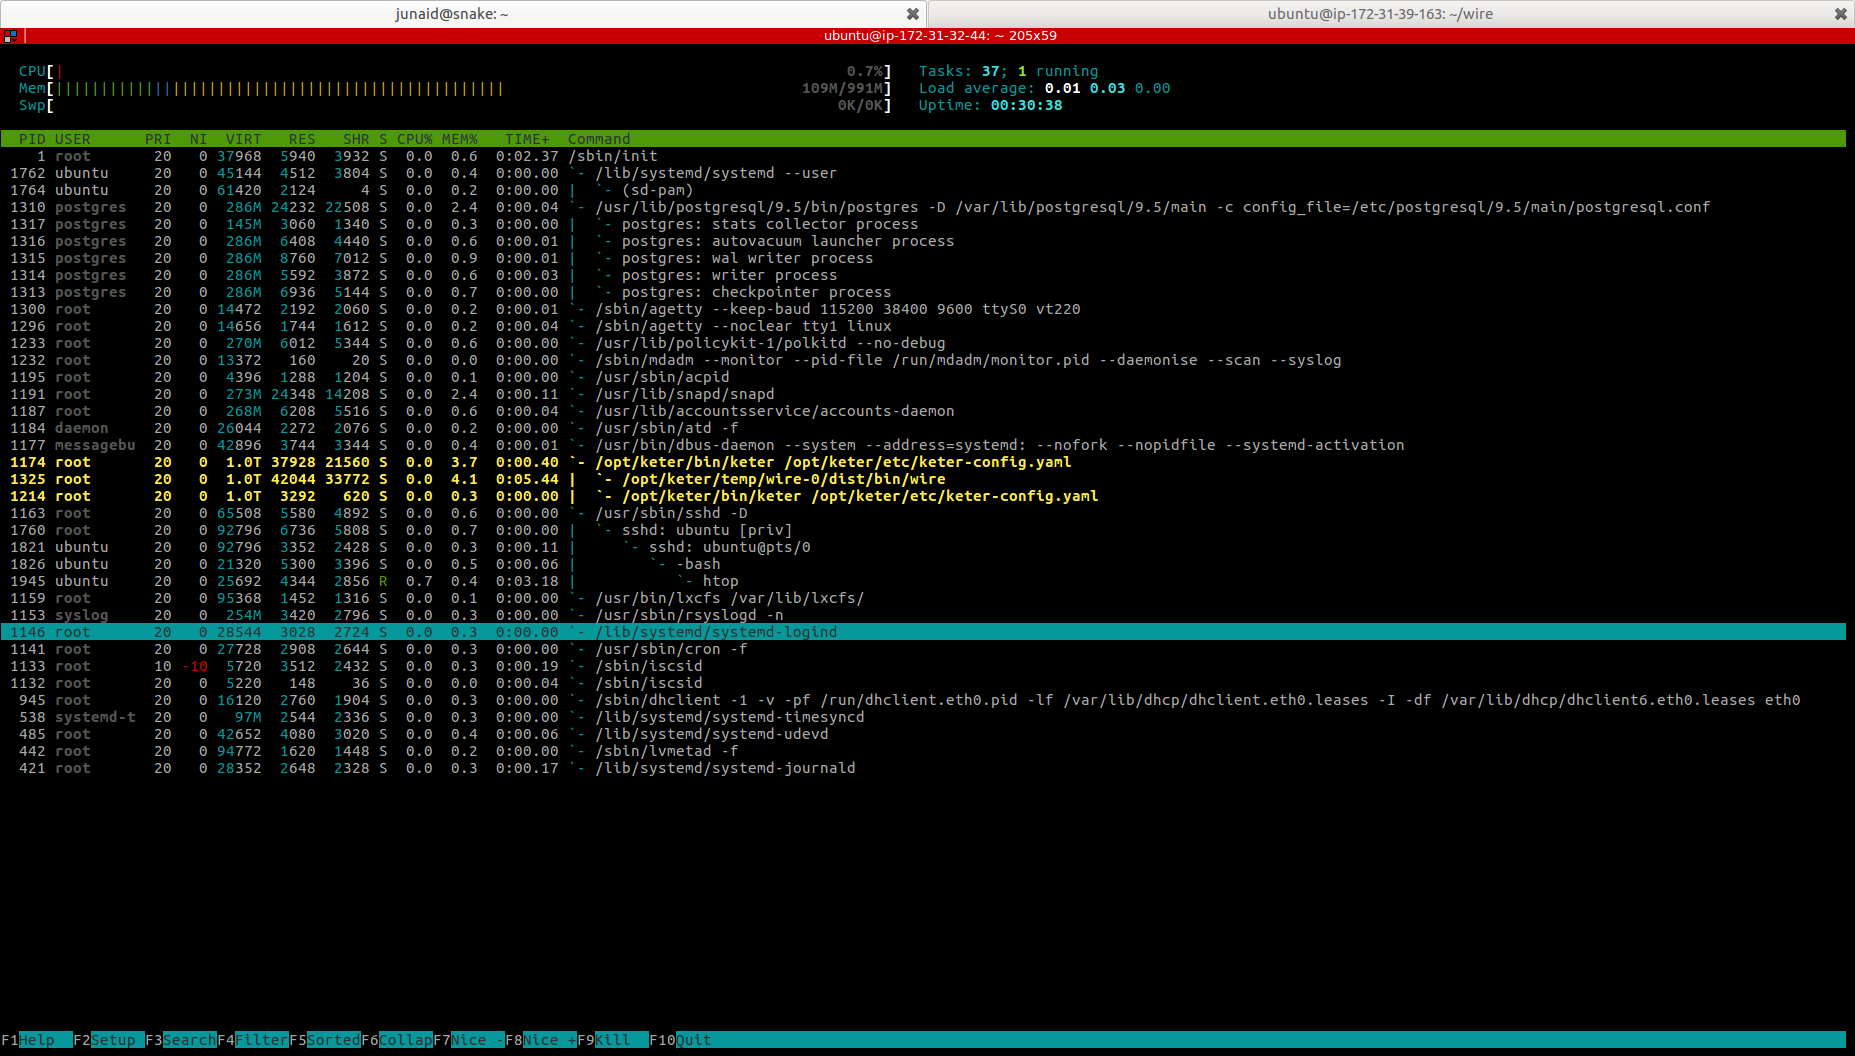
\includegraphics[width=1\textwidth]{final_report/pics/yesodIdle.png}
	\caption{Yesod htop output}
	\label{fig:yesodHtop}
\end{figure}

\begin{figure}[H]
	\centering
	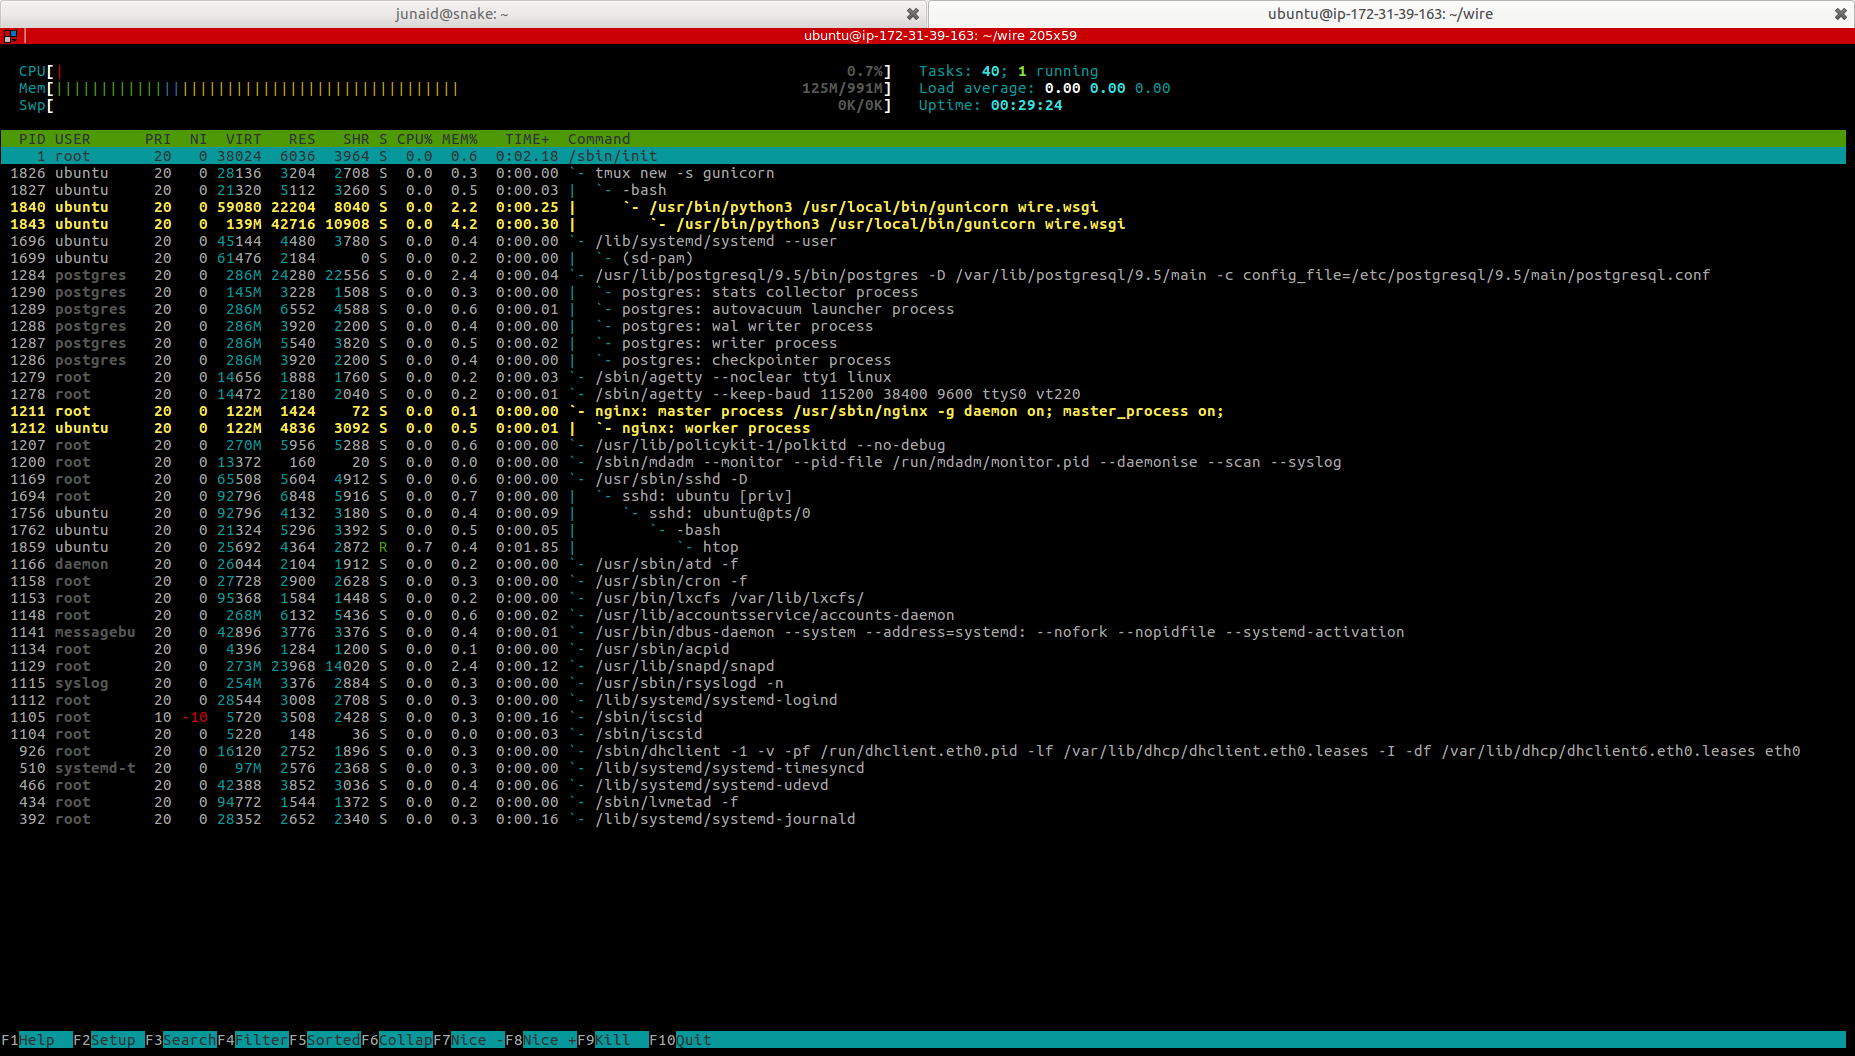
\includegraphics[width=1\textwidth]{final_report/pics/djangoIdle.png}
	\caption{Django htop output}
	\label{fig:djangoHtop}
\end{figure}

\section{Continuous Integration Build Times}

Both frameworks are stored on a git repository on GitHub. Whenever there is a
new commit, Travis CI, a continuous integration tools, starts to build
both frameworks and run tests. The tool will tell you whether or not tests
have passed. Django builds take around 2.5 minutes. Yesod builds take around
3.5-4 minutes. It should be noted that the first Yesod build took 32 minutes.
This was because the first build had to compile all the library files in the
Yesod project. Once these are compiled, they are cached, allowing them to
be used for future builds.

\begin{figure}[H]
	\centering
	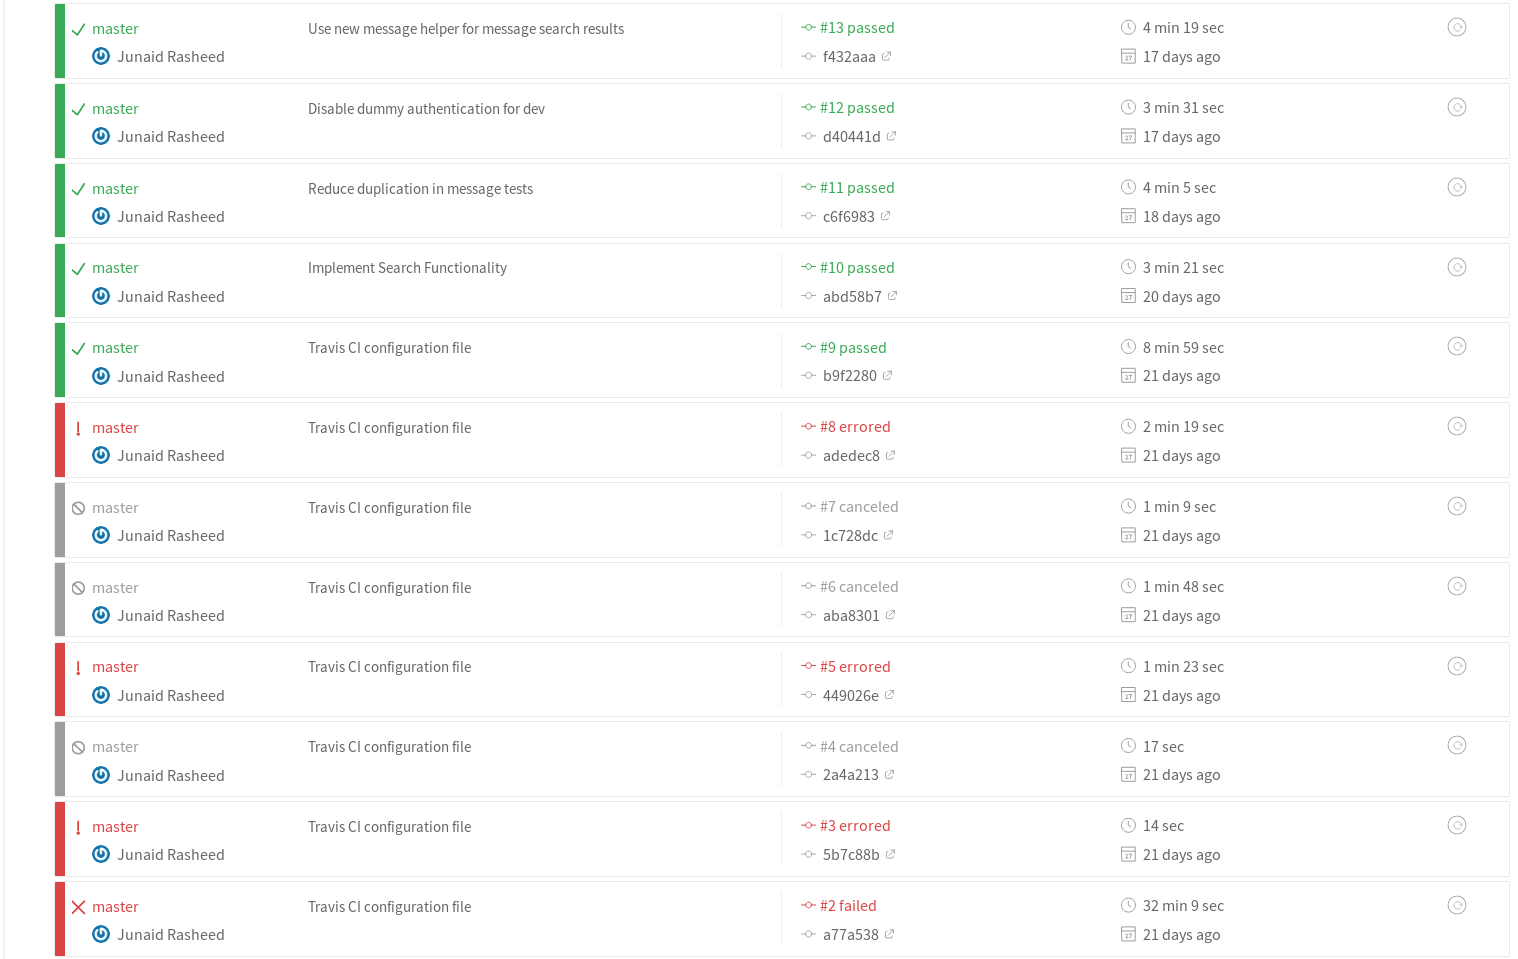
\includegraphics[width=0.9\textwidth]{final_report/pics/yesodTravis.png}
	\caption{Yesod Travis build times}
	\label{fig:yesodTravis}
\end{figure}

\begin{figure}[H]
	\centering
	
\includegraphics[width=0.9\textwidth]{final_report/pics/djangoTravis.png}
	\caption{Django Travis build times}
	\label{fig:djangoTravis}
\end{figure}

\section{Load Tests}

Load tests were ran using RedLine13 and Amazon EC2 servers. Load tests consisted of 80
users loading a specified page. Three tests were conducted. In one test, the home page
was loaded. In the two other tests, the profile page for a user who posted three
messages was loaded. Results can be found in ~\ref{tab:loadTests}

\begin{table}[H]
	\caption{Load Testing Page Load Speeds}
	\begin{center}
		\begin{tabular}{ | l | l | l |}
			\hline
			Page & Yesod (s) & Django (s) \\
			\hline
			Home & 4.96 & 5.54 \\
			Profile & 5.05 & 4.94 \\
			Profile & 4.97 & 5.13 \\
			Average & 4.99 & 5.20 \\
			\hline
		\end{tabular}
	\end{center}
	\label{tab:loadTest1}
\end{table}

\begin{table}[H]
	\caption{Load Testing Data Received}
	\begin{center}
		\begin{tabular}{ | l | l | l |}
			\hline
			Page & Yesod (MB) & Django (MB) \\
			\hline
			Home & 6.28 & 17.99 \\
			Profile & 6.76 & 18.74 \\
			Profile & 6.34 & 17.84 \\
			Average & 6.46 & 18.19 \\
			\hline
		\end{tabular}
	\end{center}
	\label{tab:dataTests}
\end{table}

\begin{figure}[H]
	\centering
	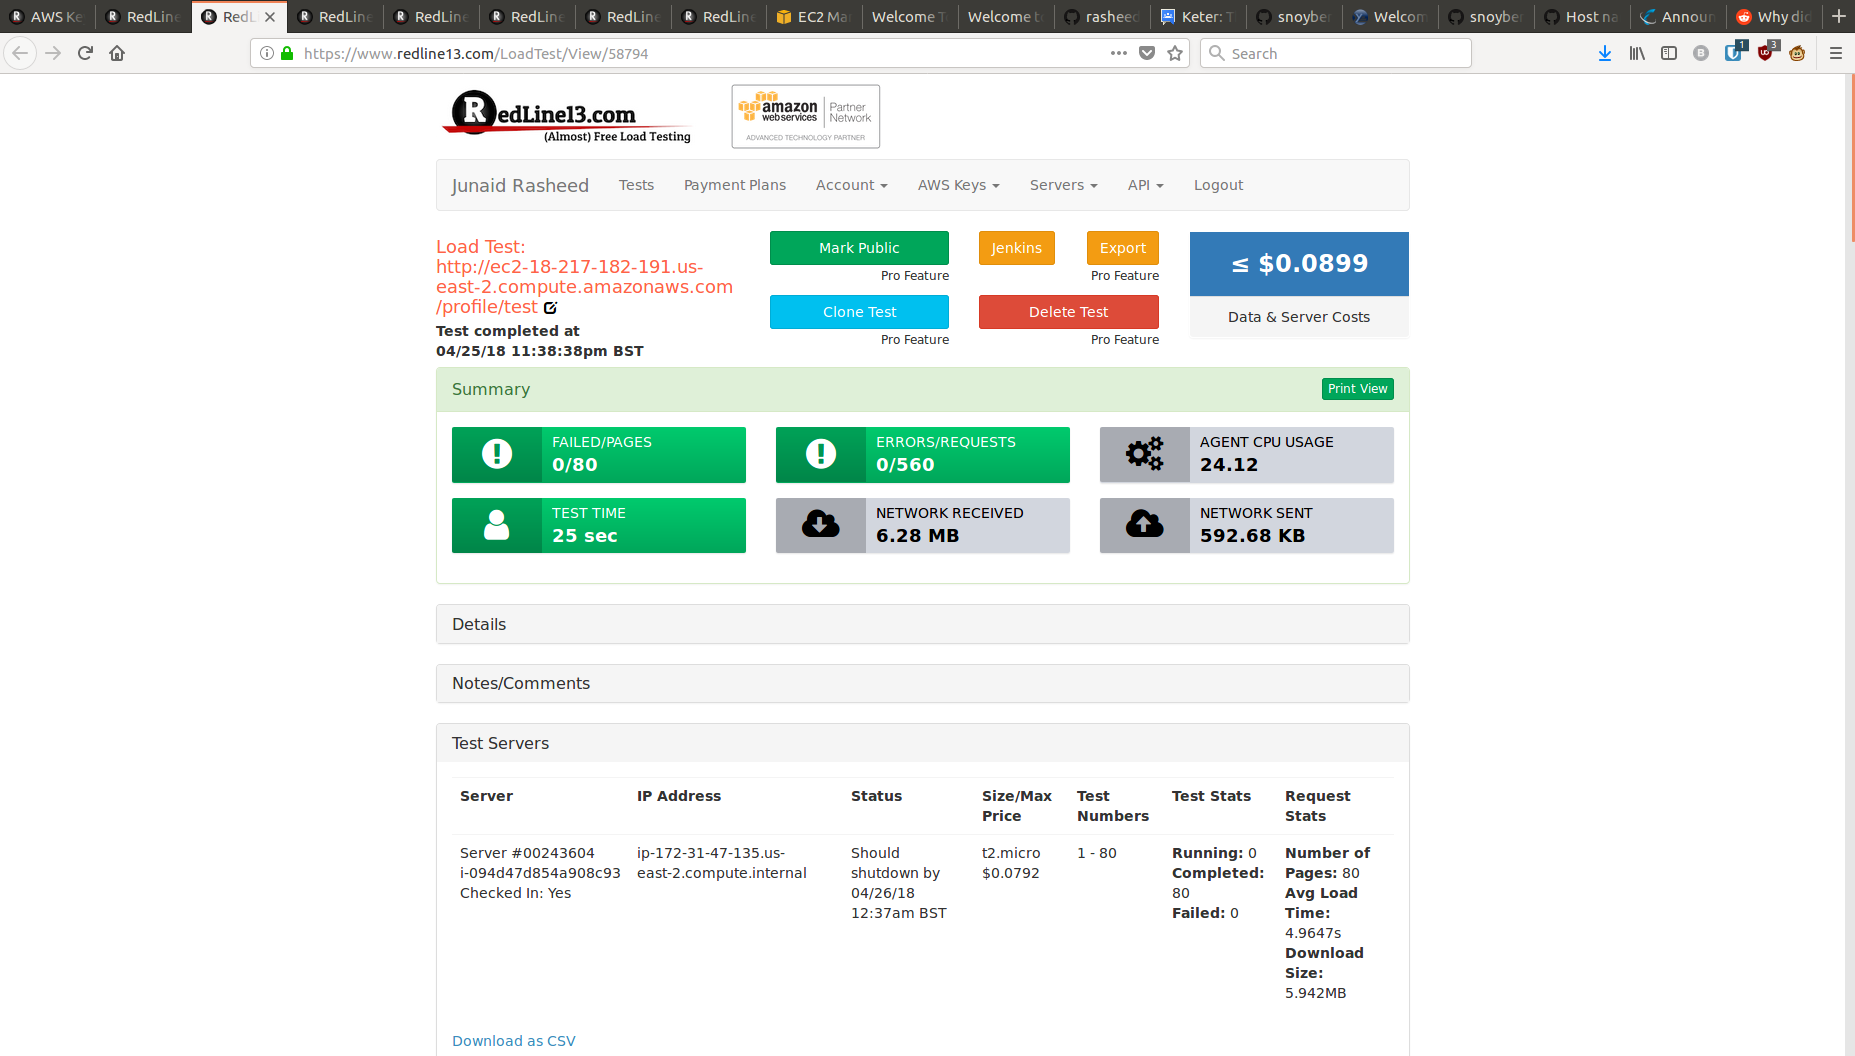
\includegraphics[width=0.9\textwidth]{final_report/pics/yesodLoadTest1.png}
	\caption{Yesod Load Test 1}
	\label{fig:yesodLoadTest1}
\end{figure}

\begin{figure}[H]
	\centering
	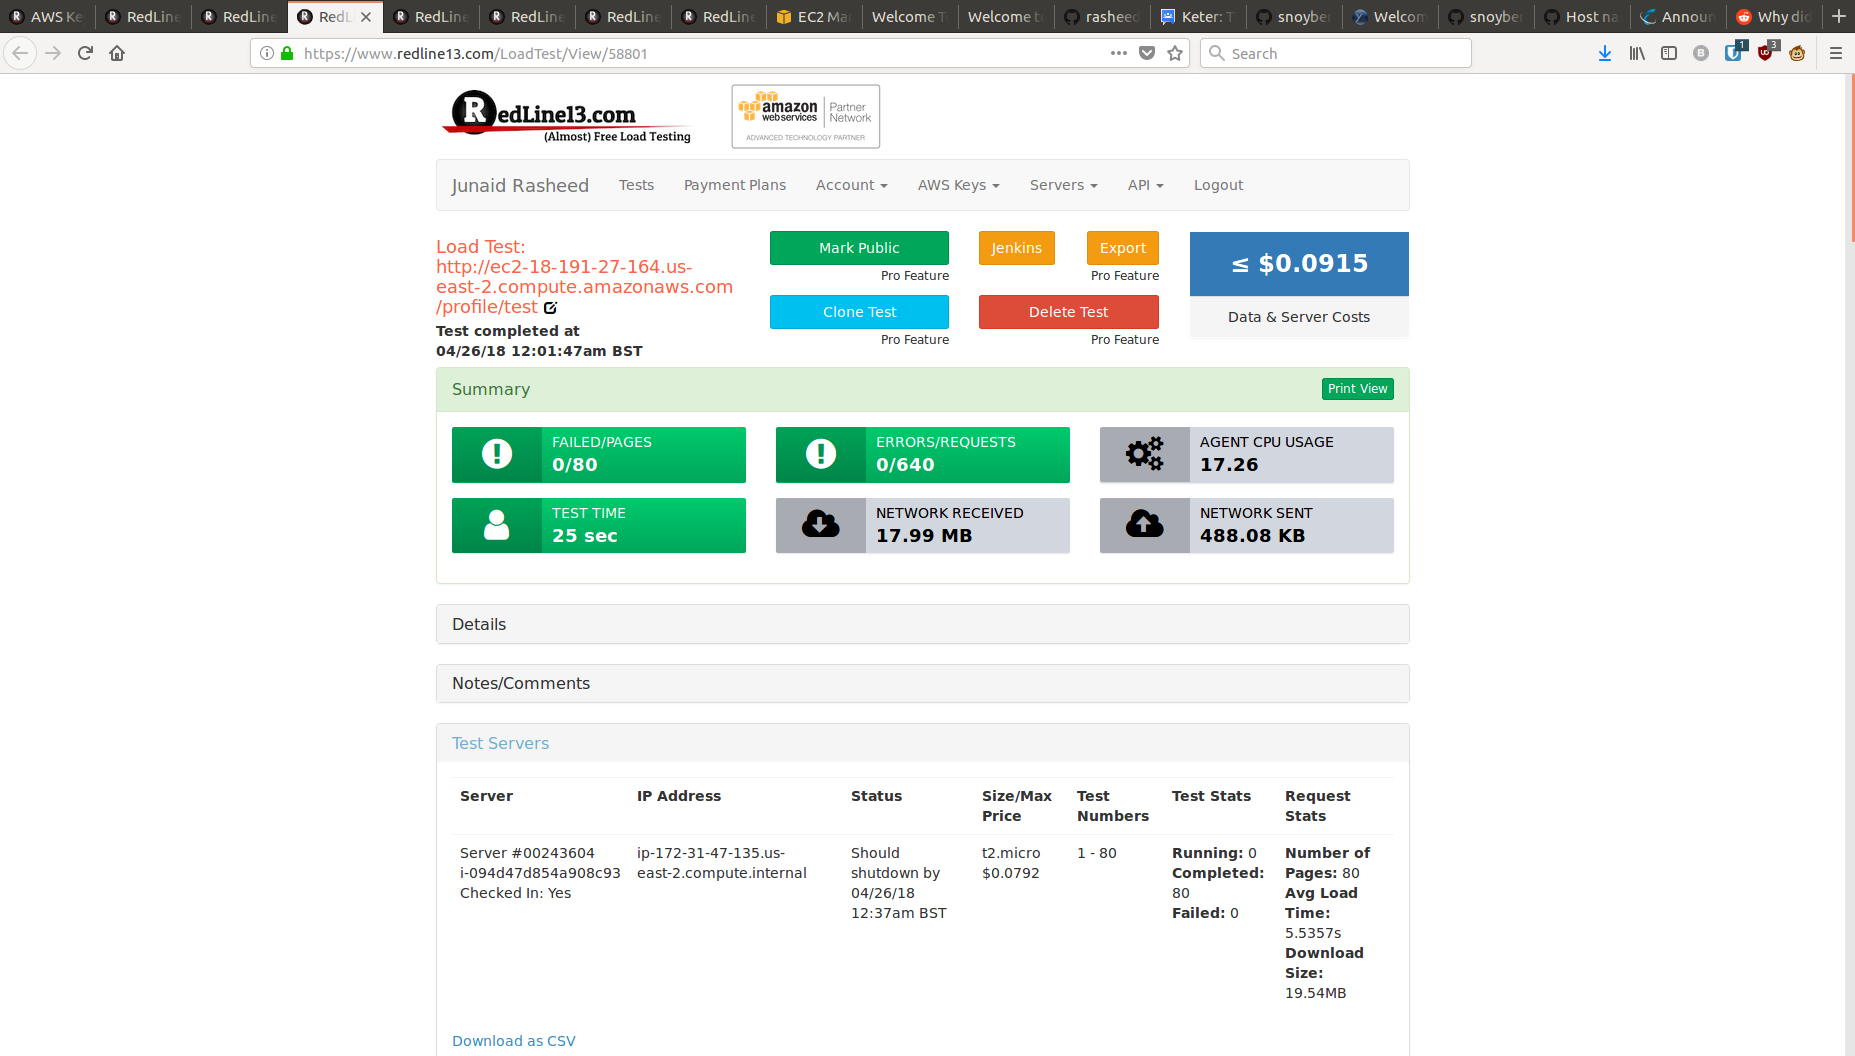
\includegraphics[width=0.9\textwidth]{final_report/pics/djangoLoadTest1.png}
	\caption{Django Load Test 1}
	\label{fig:djangoLoadTest1}
\end{figure}

\begin{figure}[H]
	\centering
	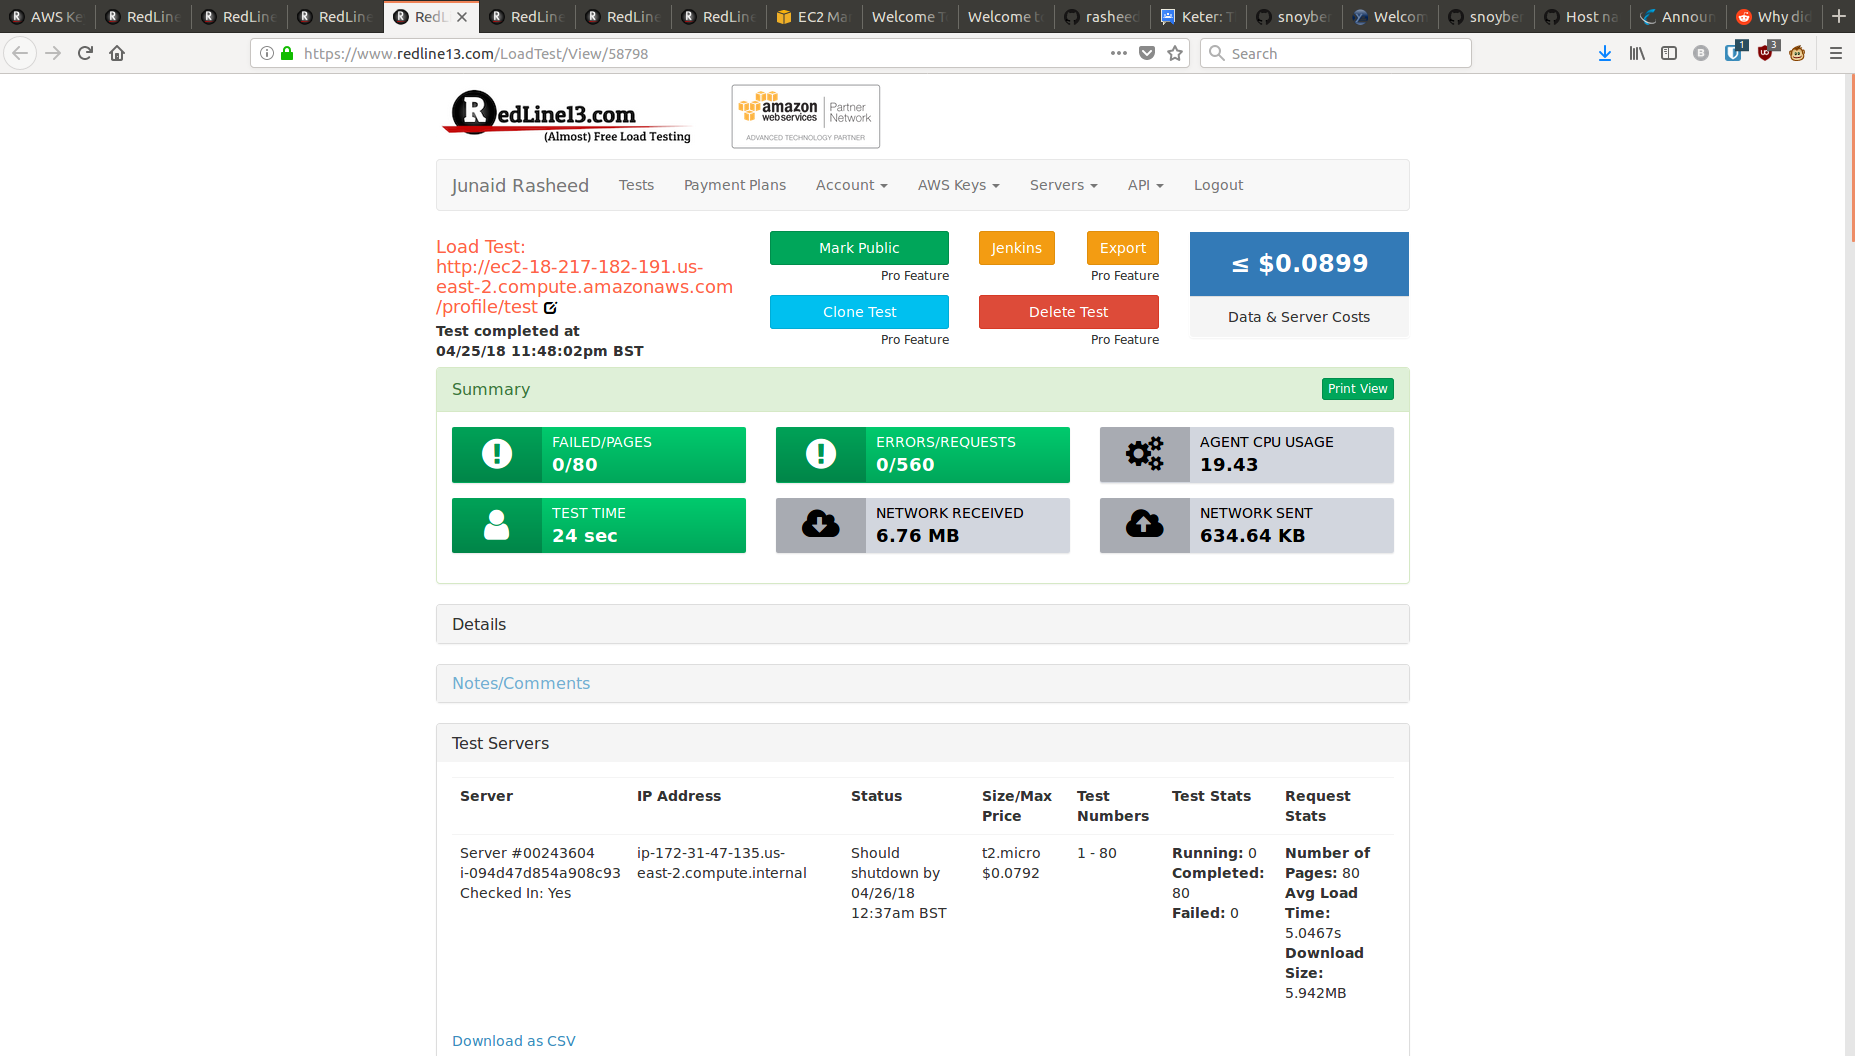
\includegraphics[width=0.9\textwidth]{final_report/pics/yesodLoadTest2.png}
	\caption{Yesod Load Test 2}
	\label{fig:yesodLoadTest2}
\end{figure}

\begin{figure}[H]
	\centering
	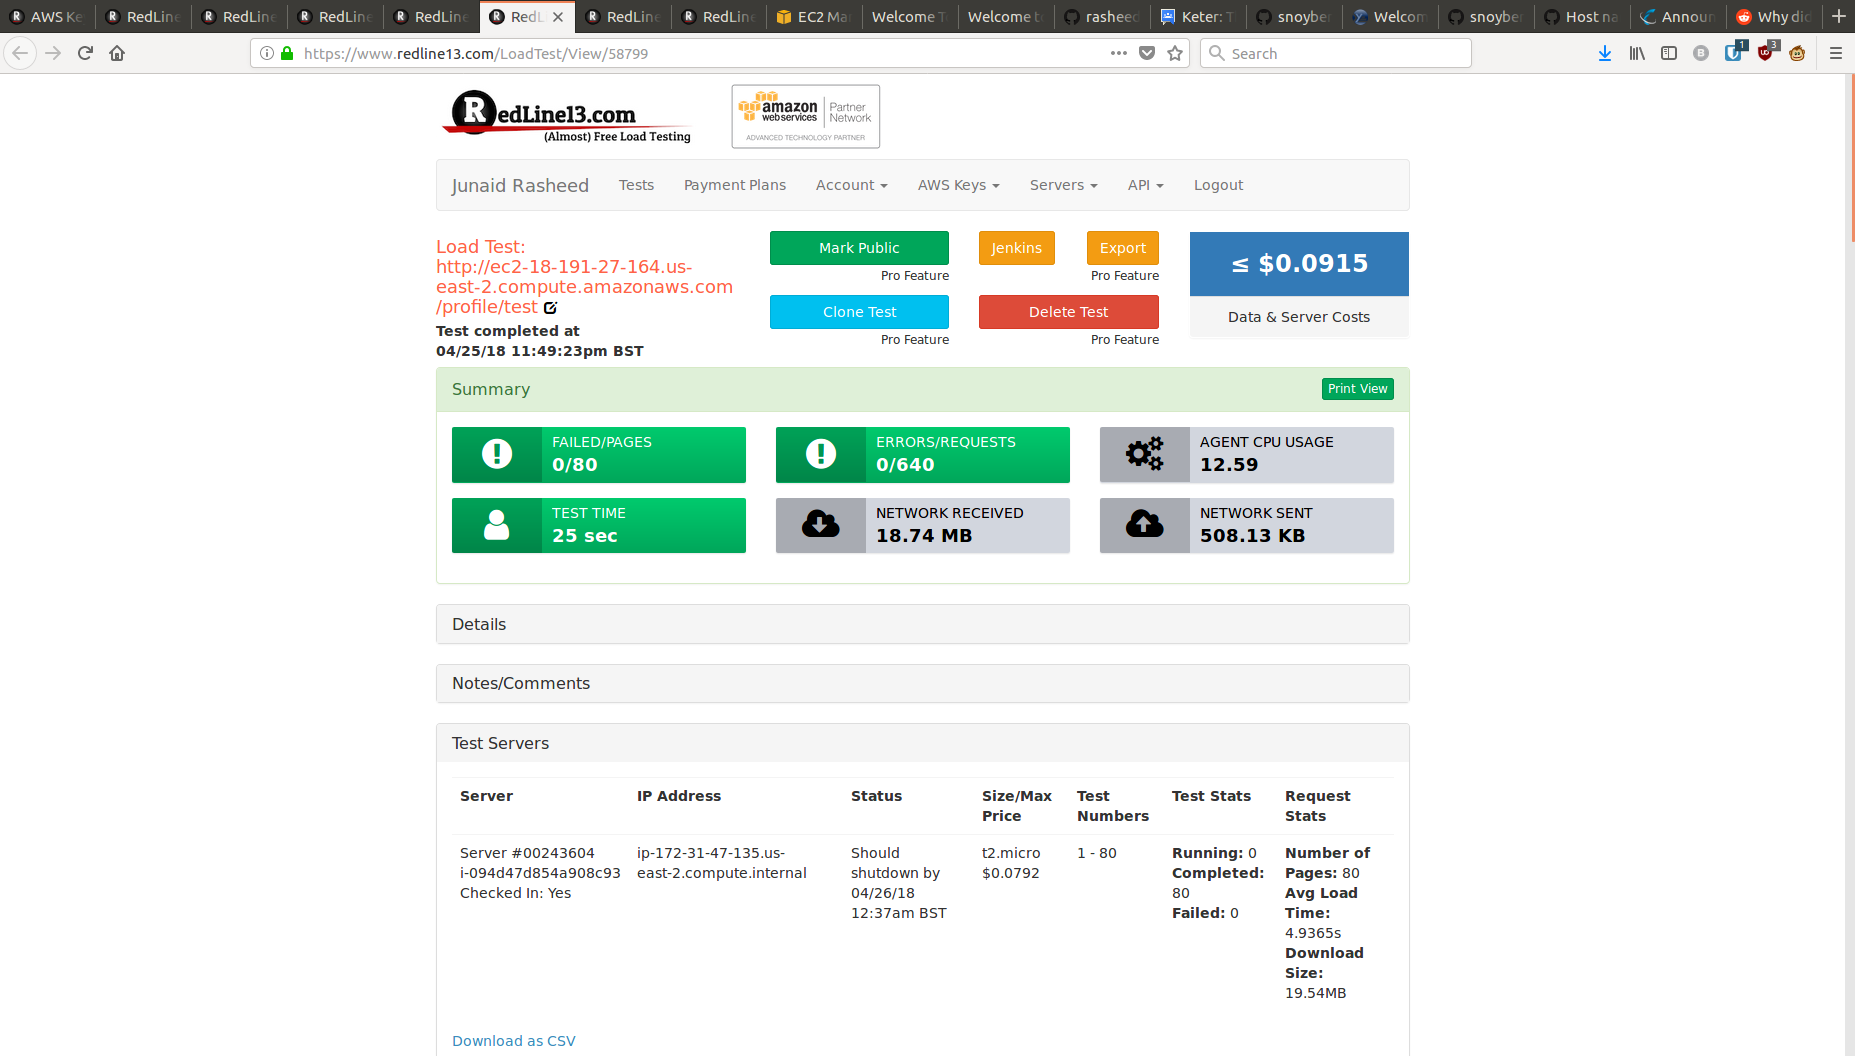
\includegraphics[width=0.9\textwidth]{final_report/pics/djangoLoadTest2.png}
	\caption{Django Load Test 2}
	\label{fig:djangoLoadTest2}
\end{figure}

\begin{figure}[H]
	\centering
	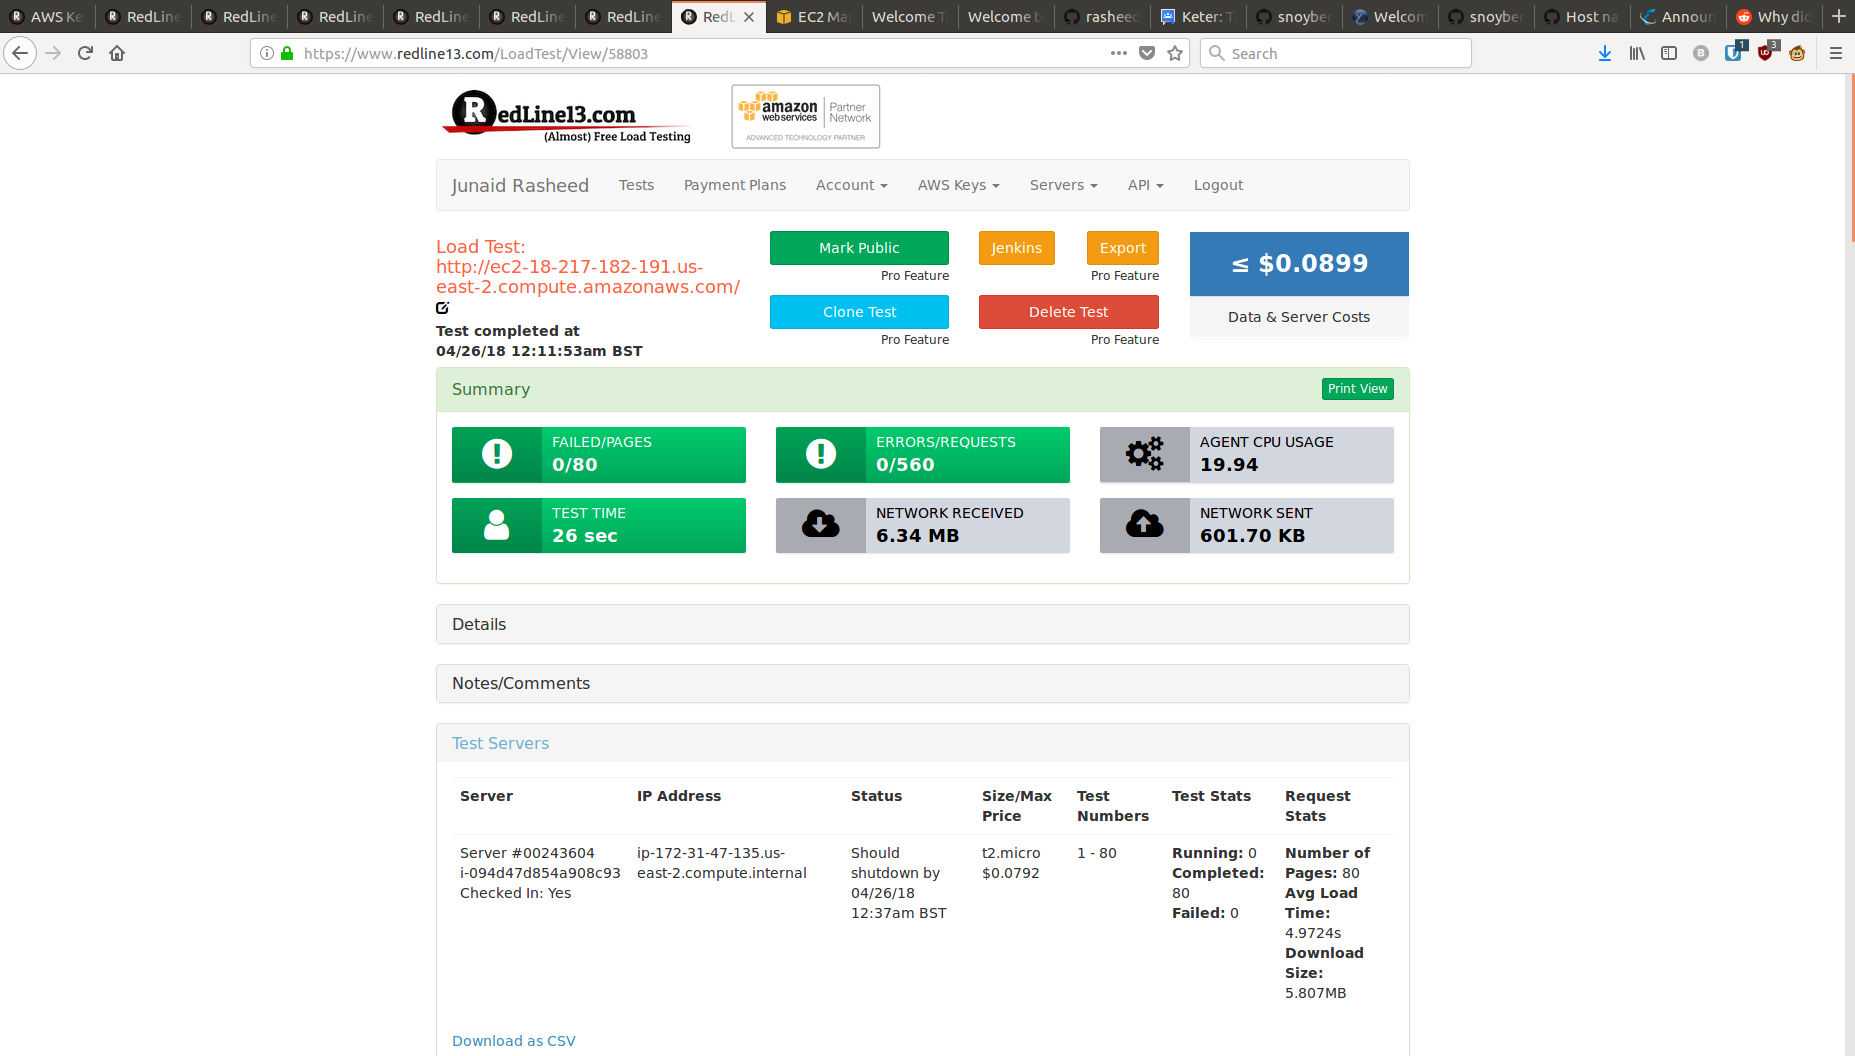
\includegraphics[width=0.9\textwidth]{final_report/pics/yesodLoadTest3.png}
	\caption{Yesod Load Test 3}
	\label{fig:yesodLoadTest3}
\end{figure}

\begin{figure}[H]
	\centering
	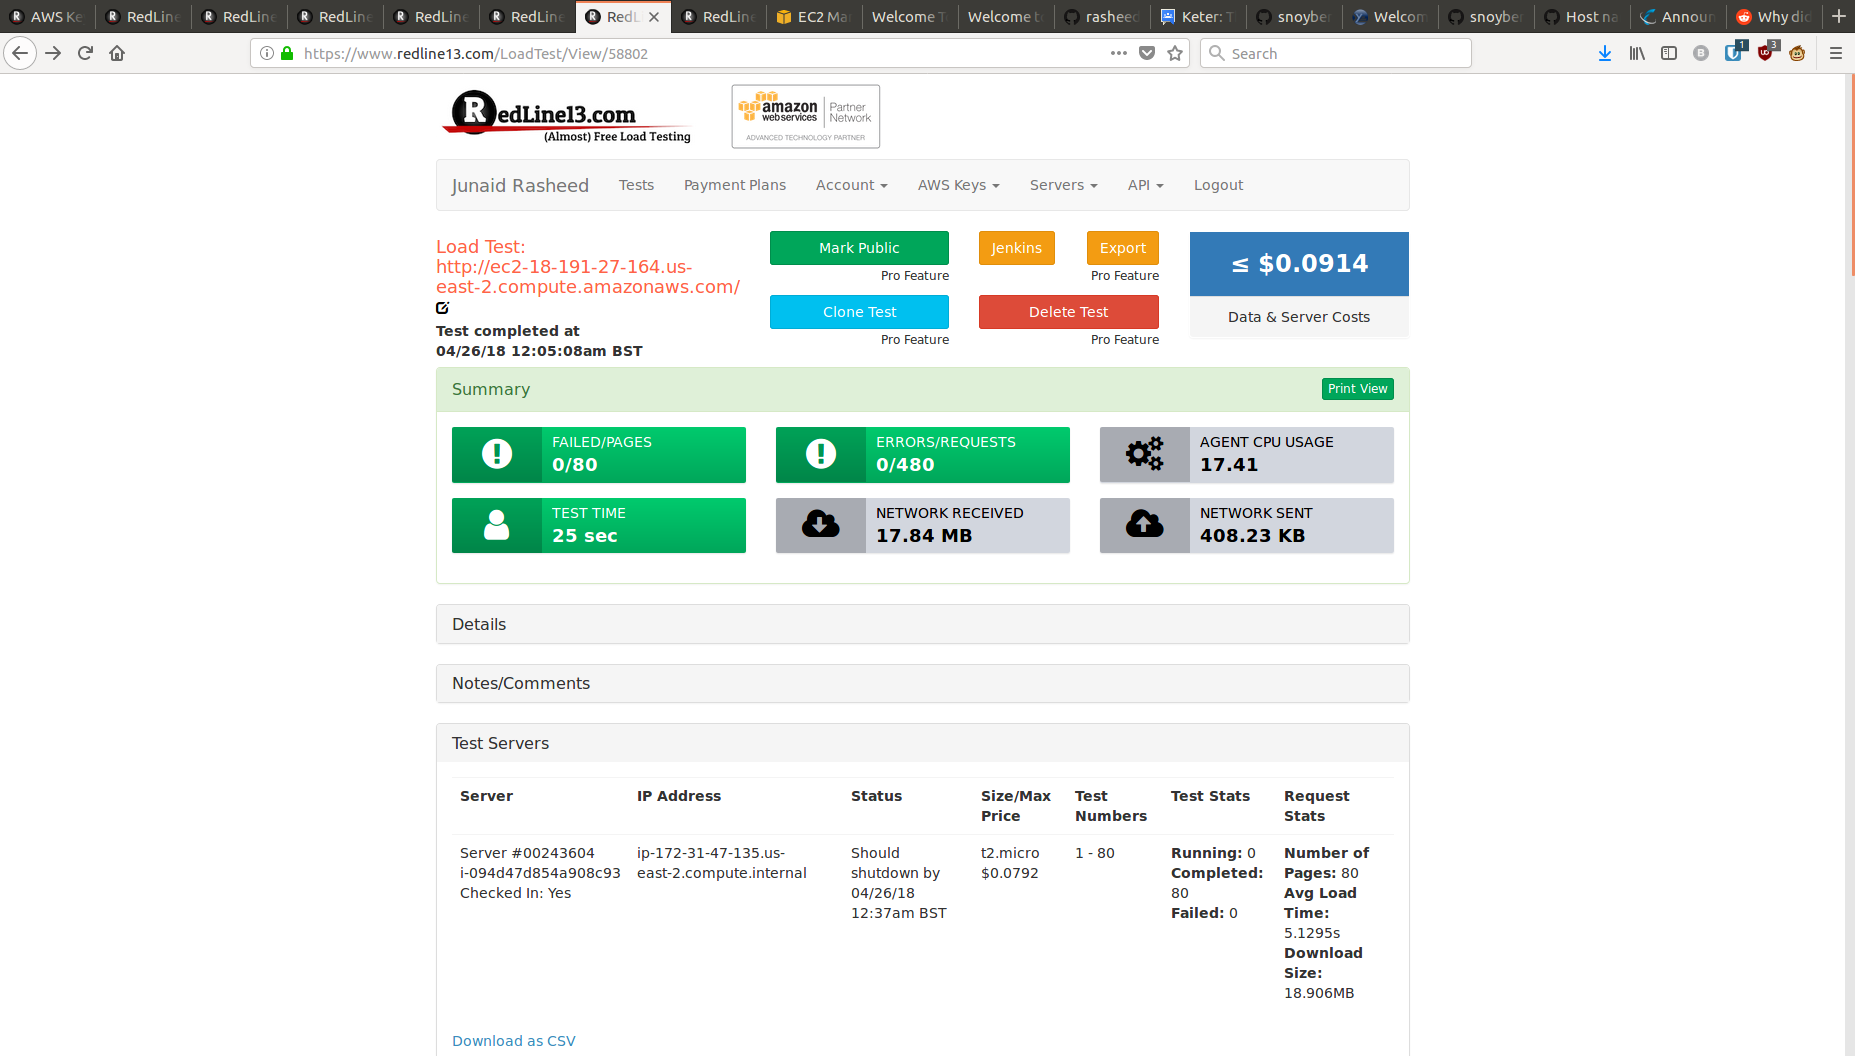
\includegraphics[width=0.9\textwidth]{final_report/pics/djangoLoadTest3.png}
	\caption{Django Load Test 3}
	\label{fig:djangoLoadTest3}
\end{figure}

\section{Introducing Realistic Errors}

For these tests, we purposefully made an error that could realistically happen.
After we made the error, we see the error messages that each framework gives us.

\subsection{Test 1}
When creating a message, try to save the form results rather than
the message extracted from the results into the database.

Yesod Results: Did not compile, unmatched type error. Tests can't be ran
as site did not compile.
Django Results: No error thrown even when submitting new message form.
Message not created. Database entry added, form data was converted to
string and added to Database. Tests passed because they were checking
the database count. This test was fixed to check the database content
as well.

\lstset{language={Haskell}}
\begin{lstlisting}[caption={Yesod Code Change},label={code:yesodTest1LC}]
	(Entity userId _) <- requireAuth
	((result, _), _) <- runFormPost $ messageForm userId
	case result of
		FormSuccess message -> do
			-- _ <- runDB . insert $ message -- original line 
			_ <- runDB . insert $ result -- new line 
\end{lstlisting}

\lstset{language={Python}}
\begin{lstlisting}[caption={Django Code Change},label={code:djangoTest1LC}]
	form = NewWireForm(request.POST)
	if form.is_valid():
		if request.user.is_authenticated:
			message = form.cleaned_data['message']
			try:
				# Message.objects.create(message_text=message, .. # original line
				Message.objects.create(message_text=form.cleaned_data, .. # changed line 1
				# Message.objects.create(message_text=form, .. # changed line 2, after previous line passed
\end{lstlisting}


\lstset{language={Haskell}}
\begin{lstlisting}[caption={Yesod Exception Message},label={code:yesodTest1Exception}]
	- Couldn't match type `PersistEntityBackend (FormResult Message)'
	with `SqlBackend'
	arising from a use of `insert'
	- In the second argument of `(.)', namely `insert'
	In the expression: runDB . insert
	In a stmt of a 'do' block: _ <- runDB . insert $ result
\end{lstlisting}

\begin{figure}[H]
	\centering
	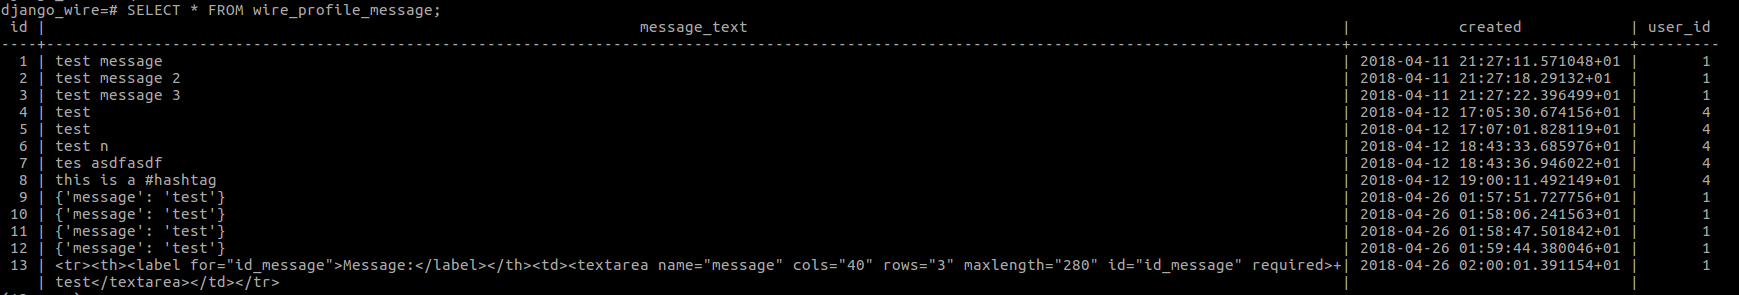
\includegraphics[width=0.9\textwidth]{final_report/pics/djangoMessageDB.png}
	\caption{Django Message Table Values}
	\label{fig:djangoMessageDBTest1}
\end{figure}

\subsection{Test 2}
Simply misspell a variable name. Most IDE tools catch this anyway but
error messages are useful to see. The misspelling was done in the code
that returns recommended users on the profile page. This code returns
data in JSON format.

Yesod: Did not compile, variable not in scope error. Compiler recommended
actual variable.

Django: AJAX request returned  a 500 error. Loading the page shows the
debug output. Exception thrown with message ``name `user' is not defined''.
Tests failed.

\lstset{language={Haskell}}
\begin{lstlisting}[caption={Yesod Code Change},label={code:yesodTest2LC}]
	Entity userId user <- requireAuth
	followers <- runDB $ selectList [FollowFollowerId ==. userId] []
	-- See: https://stackoverflow.com/questions/36727794/haskell-persistent-reusing-selectlist
	let followingIds = map (\(Entity _ (Follow _ followingId)) -> followingId) followers
	users <- runDB $ selectList [UserUsername !=. userUsername user, UserId /<-. followingIds] [LimitTo 5]
	let cleanUsers = map (\(Entity uid (User uname _ _)) -> (object ["id" .= uid, "username" .= uname])) users
	-- returnJson cleanUsers -- original line
	returnJson cleanUser -- new line
\end{lstlisting}

\lstset{language={Python}}
\begin{lstlisting}[caption={Django Code Change},label={code:djangoTest2LC}]
	if request.user.is_authenticated:
	follow_query = Follow.objects.filter(follower_id=request.user)
	users = User.objects.filter().exclude(id=request.user.id).exclude(username=excluded_username)\
		.exclude(followed_user__in=follow_query).values('username')[:5]
	# return JsonResponse(list(users), safe=False)  # original line
	return JsonResponse(list(user), safe=False)  # new line
\end{lstlisting}

\lstset{language={Haskell}}
\begin{lstlisting}[caption={Yesod Exception Message},label={code:yesodTest2Exception}]
	Variable not in scope: cleanUser
	Perhaps you meant `cleanUsers' (line 19)
\end{lstlisting}

\lstset{language={Python}}
\begin{lstlisting}[caption={Django Exception Message},label={code:djangoTest2Exception}]
	NameError at /get-recommended-users/test
	name `user' is not defined
\end{lstlisting}

	
\chapter{Project Diary}
\section{Meeting 1 - 3rd October 2017}

\subsection{Meeting Notes:}

\subsubsection{Books}

Real World Haskell\\
Haskell from first principles (haskellbook.com)\\
Web application development with Haskell and Yesod (out of date)

\subsubsection{Frameworks / Tools}

Haskell Servant package\\
Snap is alternative to Yesod\\
ghcjs haskell to js\\
haskell stack tool\\
hackage is like npm. Stack can use hackage.\\
Stackage is like stack on top of hackage\\
Use the latest LTS version of haskell from stackage\\
Atom could be useful with their plugins, compare with plugins available for code\\
ghc-mod available for haskell in atom, helpful when developing\\
ide-haskell, linter\\
There is a Haskell plugin for intellij which may work. Good because I would be familiar with the IDE.

\subsubsection{Comparing the two frameworks}

\begin{itemize}
  \item Maintainability
  \begin{itemize}
    \item Make a change to both
  \end{itemize}
  \item Performance
  \item Scalability - could use tools, hard to do on your own
  \item People say Haskell is easier to write code with, less time debugging, once learnt
  \begin{itemize}
    \item We could test this. How much the type checking helps. The different tools available
    \item Can't use line by line debugging
  \end{itemize}
\end{itemize}

\subsubsection{Plan for next meeting}

Do as much as possible for now\\
Come up with rough project definition form\\
Go through some haskell tutorials, haskellbook.com is recommended

\section{Meeting 2 - 12th October 2017}

\subsection{Meeting Notes:}

Look into getting GHC mod compile on save\\
Get the project proposal doc ready for next week\\
Learn Django and get it installed on the laptop\\
Make a basic page in Django and Haskell

\section{Meeting 3 - 19th October 2017}

\subsection{Meeting Notes:}

Carry on with the Haskell Programming from First principles book\\
Have some planning for the twitter clone ready

\section{Meeting 4 - 24th October 2017}

\subsection{Meeting Notes:}

Set up a basic homepage in Yesod and Django. Do this over the weekend.\\
Have a play around with the yesod site that’s provided to see what you can focus on.\\
Carry on with the book\\
Setup Docker/Vagrant if you have time at the end, for instructions on setting up the repo\\
Topics important for yesod
\begin{itemize}
  \item Quasi quotes, provided by yesod
  \item Yesod Typeclass could be useful to know
\end{itemize}

\section{Meeting 5 - 10th November 2017}

\subsection{Meeting Notes:}

I’ve created the homepages in both yesod and django. I’ve used tests in django to test a basic app not related to the project

Next week, I want to ensure both home pages are the same and to create tests in both frameworks. I want to progress more through the yesod and haskell book.
Create User models in both yesod and django and create tests for them.

\section{Meeting 6 - 16th November 2017}

\subsection{Meeting Notes:}

I’ve created the homepages in yesod and django and ensured that they both have the same content and styling.

For django, I have added the functionality to allow users to create accounts and log in. I have added unit tests for this and they all pass.

For yesod, I have added the latest version of jquery and bootstrap to the project. I have tried to complete the user account functionality but I am blocked. I am trying to import yesod-auth-hashdb but cannot figure out how to do it. There is some documentation showing how to edit the cabal file but this is overwritten during the build, I believe the data comes from package.yml. Editing package.yml causes strange errors when I try to build the project but I don’t think I am doing it in the correct manner. Need to figure out how to edit the package.yml, edits would result in errors on my computer.

For next week, I want to fix the weird error and get some tests up.

Things to try to resolve the error, try to reproduce it on normal ubuntu. If you can’t resolve it, report it to yesod.

\section{Meeting 7 - 23rd November 2017}

\subsection{Meeting Notes:}

I’ve resolved the random error we had last week.\\
I’ve imported hashdb and have added functionality for users to create accounts and login on the yesod site.\\
Yesod forms rely on bootstrap 3, so downgraded from bootstrap 4 (beta) to 3.

For next time...\\
I want to figure out how to concatenate a Text data variable in Yesod. Have to figure out how to deal with overloaded strings?\\
Finish the user authentication functionality. Show appropriate messages and add extra validation to the yesod form (unique user and email, min and max length of fields).\\
Create tests for the user authentication functionality.\\
Change the forms on Django to use their form model rather than a HTML form. This will let me compare the pros and cons of Django’s and Yesod’s forms.\\
If there is time, add functionality to allow users to post messages. These messages should be saved in the database so that the user can see all the messages they’ve posted when they log in.

The user post message page should use ajax so when they post a message, the part of the div will just reload rather than the whole page.

\section{Meeting 8 - 14th December 2017}

\subsection{Meeting Notes:}
On the yesod site:\\
Have some tests working\\
Users can post messages, be signed up, see other users messages\\
Have some tests working, this is WIP

For next time…\\
Get Django messages working\\
Try to get ajax working on both sites, see https://www.yesodweb.com/blog/2013/02/ajax-with-scaffold

Interim report plan
\begin{itemize}
  \item Intro
  \item Explain the choices of yesod and django
  \item Do some initial comparisons of the site
  \item My experiences with developing on both sites, what I found easy and hard on the different frameworks.
  \item Advantages and disadvantages of both frameworks.
\end{itemize}

\section{Meeting 9 - 1st February 2018}

\subsection{Meeting Notes:}
Worked mainly on the Django site. I have the messages working and have began comparing features between two sites such as
\begin{itemize}
  \item The implementation of Handlers/Routes
  \item The way you can pass variables to templates
  \item How Haskell's 'maybe' reduces the number of errors you need to catch
  \item the ways you can implement AJAX in both frameworks
\end{itemize}

In the near future, refactor the messages implementation to use AJAX for retrieval of messages and creating new messages. This refactoring will help compare the ease of modifiability of both of these frameworks.\\
Whenever you come across a difficult error, try to compare the process of debugging in both frameworks.\\
Remember to focus on using different parts of the framework than just implementing new features on the site.\\
Try to resolve the textarea problem. If you can't send a screenshot of the error.\\

\section{Meeting 10 - 15th February 2018}

\subsection{Meeting Notes:}
Created AJAX functionality for getting messages

Resolved issue with using single template for profile by declaring the form stuff even if isCurrentUse is false, this is fine

\subsubsection{What needs to be done}

Add more tests this weekend for both frameworks. Does Haskell's type checking mean we need fewer tests compared to Python?

\subsubsection{What to look at for evaluation}

Evaluate:
\begin{itemize}
	\item{The ease of writing tests}
	\item{In python, you need lots of testing because there's no static type checking}
	\begin{itemize}
    	\item{Does this mean you need less tests in Haskell}
    	\item{Does this mean tests are easier to write in Haskell, or in Python because tests are more important in Python so they'd be easier to use}
	\end{itemize}
	\item{What types of tests are important in the haskell world}
	\item{Some tests are unneeded for Haskell}
	\item{Is it cheaper to build a bullet proof app in Haskell or Python, maintainability? etc}
\end{itemize}

Amount of users in Django makes it easier to find problems that others have experineced

Amount of users in Django means more tools for Django but this is improving on the Haskell on the side

The Yesod book written by the creator of Yesod is pretty good

Some of the problems written by people using Yesod are more detailed, users are probably more experienced in the programming world? more academic?

Evaluate the ease of adding a new feature after the site is complete

Evaluate how quick it is to debug something

Built in compiler and type checking in Haskell is very useful when debugging

Evaluate page load speeds, is Python slower because it runs the interpreter every time?

Scalability if you can

Some quantitative data?

Explain to the reader why some things make a big difference
\begin{itemize}
    \item{How long it takes to get a reliable application}
    \begin{itemize}
        \item{Length of tests? Number of tests? Instances where types catch important errors? These are very useful}
        \item{Times where the type checking or other similar features got in your way?}
        \begin{itemize}
            \item{E.g. profile page was easier to code in Python, this was because of Haskell checking the scoping}
		\end{itemize}
	\end{itemize}
\end{itemize}
\section{Meeting 11 - 22nd March 2018}

\subsection{Meeting Notes:}
Implemented type safety for some URLs

\begin{itemize}
  \item{How much does it help with testing / debugging?}
  \item{Does this reduce the amount of code you need (to check parameter types, etc.)}
\end{itemize}

Joins cannot be done with Yesod Persistent (alternative pseudo SQL available) but restructuring
logic may be more efficient than joins.

\subsubsection{Plan for the holidays and beyond}
\begin{itemize}
  \item{Finish the functionality of both websites by the end of week 2 of the holidays}
  \item{Produce a report by the end of week 3 of the holidays}
  \item{Get feedback and produce another version of the report the first week back from the holidays}
  \item{Get more feedback and produce a final version of the report the second week after the holidays}
\end{itemize}

\section{Meeting 12 - 19th April 2018}

\subsection{Meeting Notes:}
Report draft, hand in by this weekend.

Book in a meeting on Tuesday to discuss the report.

Simulate mistakes and see how the Haskell compilers help

Argue against how the compiler may make you write unnecessary code

\begin{itemize}
  \item{Haskell version, I couldn't do something like if not null, ignore the block}
  \item{You can try to use an undefined and force an exception}
  \item{You can do something like ``Error - (loc) shouldn't happen''}
\end{itemize}

Type safety saved a lot of time with checking variable types

But people like python because of the lack of type checking

It may be faster to ignore types when developing but it could cause problems later on

Think about separating language and framework

For this report, it's more useful to focus on the framework, but think about anything to do with the language

For example, static type checking is to do with Haskell rather than Yesod

In the yesod-test package, you can use HTML selectors. That makes testing static content easy.

Django, you can test HTML page but selectors are not implemented. (If html page contains this string).

If you have time after getting the report done...

Load testing, deploy both apps to the same environment. Is there a tool for it. Send 
multiple queries from multiple machines, time responses.

If no tool, you can try requests from just your own machine.
If you can't get it on Heroku, set up a VM.

Test the ease of deployments for both frameworks. Test the actual production mode, not dev mode.

\section{Meeting 13 - 24th April 2018}

\subsection{Meeting Notes:}
Entity relation diagram.

Redo tests on EC2 instances.

For research reports
\begin{itemize}
  \item State objective, hypothesis, search question.
  \item Methodology, development (testing, iterative development, conntinous integration)
  \item Mention websites as explicit deliverables that support the comparison.
  \item Comparison methodology, what do frameworks give you to support TDD.
  \item Evaluation methodology, deploy, page load speeds, load speeds, documentation.
\end{itemize}

Background chapter, expand on Yesod and Django components. 
Some diagrams would be nice.


\section{Meeting 14 - 26th April 2018}

\subsection{Meeting Notes:}


For the networking test where you mention that Django uses more data,
use the network tab on the browser to confirm this. If you load
the site in Yesod, the data loaded is lower and then it's compressed.

Fix lstlisting, set language before code blocks.

When Yesod throws errors, say runtime error, with a compiler message.

texcel, you can use macros. Could make font for code smaller.
Reformat the code blocks to be easier to read.
Any case against the types. Early profile page was one request/view. This meant that
there was some extra Haskell code that had to be written.

Last section, fix typo `Yesod being less resource intensive than Yesod.', wrong
your.

Small section that talks about how you made a functional, actually usable,
site. Site is realistic, which gives us a useful way to evaluate the frameworks.
This could be before the testing method.

Amazon monitoring is only available in five minute intervals (free usage limit).

A refactor at the end would have been useful to evaluate at the end. Does
the more rigid structure of the Haskell program help with refactoring?
Haskell compiler would guide you on what needs to be changed after a
small change.

Conclusion
Summarise the entire report, half a page, a side.

Get rid of some of the more uninteresting website images.

A useful diagram would explain the architecture of each framework.

\section{Project Definition Form}

\subsection{14th October 2017}

First draught written up and sent to tutor via email for feedback

\subsection{15th October 2017}

Tutor feedback implemented

\subsection{19th October 2017}

Tutor and I signed form. Form is submitted electronically via Turnitin

\section{Interim Report}

\subsection{18th January 2018}
Interim report started and then finished

\subsection{19th January 2018}
Sent Ethics form to tutor

Proof-read and submitted the interim report

\section{Software Development}

This section records the development lifecycle of the Django and Yesod sites. More detailed commit messages
can be found by running a \textit{git log} on the git repo for both sites.

\subsection{Yesod Site}

\subsubsection{1st November 2017}
Created a basic homepage and a vagrantfile.

\subsubsection{23rd November 2017}
Implemented Login and Signup functionality

\subsubsection{11th December 2017}
Created a profile page

\subsubsection{14th December 2017}
Implemented message creation functionality and added some tests

\subsubsection{15th February 2018}
Modified profile page to retrieve messages using AJAX

\subsubsection{19th March 2018}
Implemented functionality to show other registered users on the profile page

\subsubsection{20th March 2018}
Basic functionality to follow users implemented

\subsubsection{21st March 2018}
Refactor profle page and follow functionality to use type safe URLs

\subsubsection{22nd March 2018}
Added functionality to allow users to follow eachother through normal usage of the site.
Previously, users had to type in a URL to follow a user

\subsubsection{31st March 2018}
Refactored profile page. Separated pages used for logged in and anonymous users, reducing
complexity. Refactoring also increased use of type safe URLs in the profile page and
when posting messages.

\subsubsection{1st April 2018}
Updated stack resolver to latest point release for current resolver, ensuring we have
the latest compatible updates for our packages. Fix some bugs and add tests.

\subsubsection{2nd April 2018}
Added tests for all route handlers and integrate tests with Travis CI.

\subsubsection{4th April 2018}
Implemented search functionality

\subsubsection{5th April 2018}
Tested the search functionality

\subsubsection{6th April 2018}
Added latest posted messages to the homepage and used a previously created datatype
to help display posted messages on the frontend.

\subsubsection{7th April 2018}
Added hashtag functionality and fixed some bugs on the profile page. Hashtagged messages
appear on the homepage.

\subsubsection{10th April 2018}
Added yesod prefix to database names so that the Yesod server can be ran the same
time as the Django server.

\subsubsection{11th April 2018}
Removed unneeded visit button on profile page.

\subsubsection{13th April 2018}
Improved ordering of messages posted by other uses on your feed.

\subsection{Django Site}

\subsubsection{9th November 2017}
Created the homepage and a vagrantfile.

\subsubsection{14th November 2017}
Implemented login and signup functionality

\subsubsection{15th November 2017}
Refactored authentication functionality to use Django's built in models rather than custom models.

\subsubsection{31st January 2018}
Implemented profile page and message creation functionality.

\subsubsection{10th April 2018}
Downgrade Django bootstrap version to bootstrap 3. This is the version used by Yesod so using
version 3 reduces the amount of template work to do which does not provide much insight
into the benefits of either framework.

Implemented breadcrumbs and a base template file that all other template files use.

\subsubsection{11th April 2018}
Added AJAX functionality to the profile page.

\subsubsection{12th April 2018}
Completed the profile page and added search functionality

\subsubsection{13th April 2018}
Added tests and fixed any bugs discovered. Latest message and hashtagged messages added to the homepage.

\section{Project Diary Final Report}

\subsection{20th April 2018}
Started write-up of the final report

\subsection{23rd April 2018}
Run experiments on Yesod and Django sites, as planned.
Completed first draft and sent to tutor for feedback



\chapter{Ethics Form}
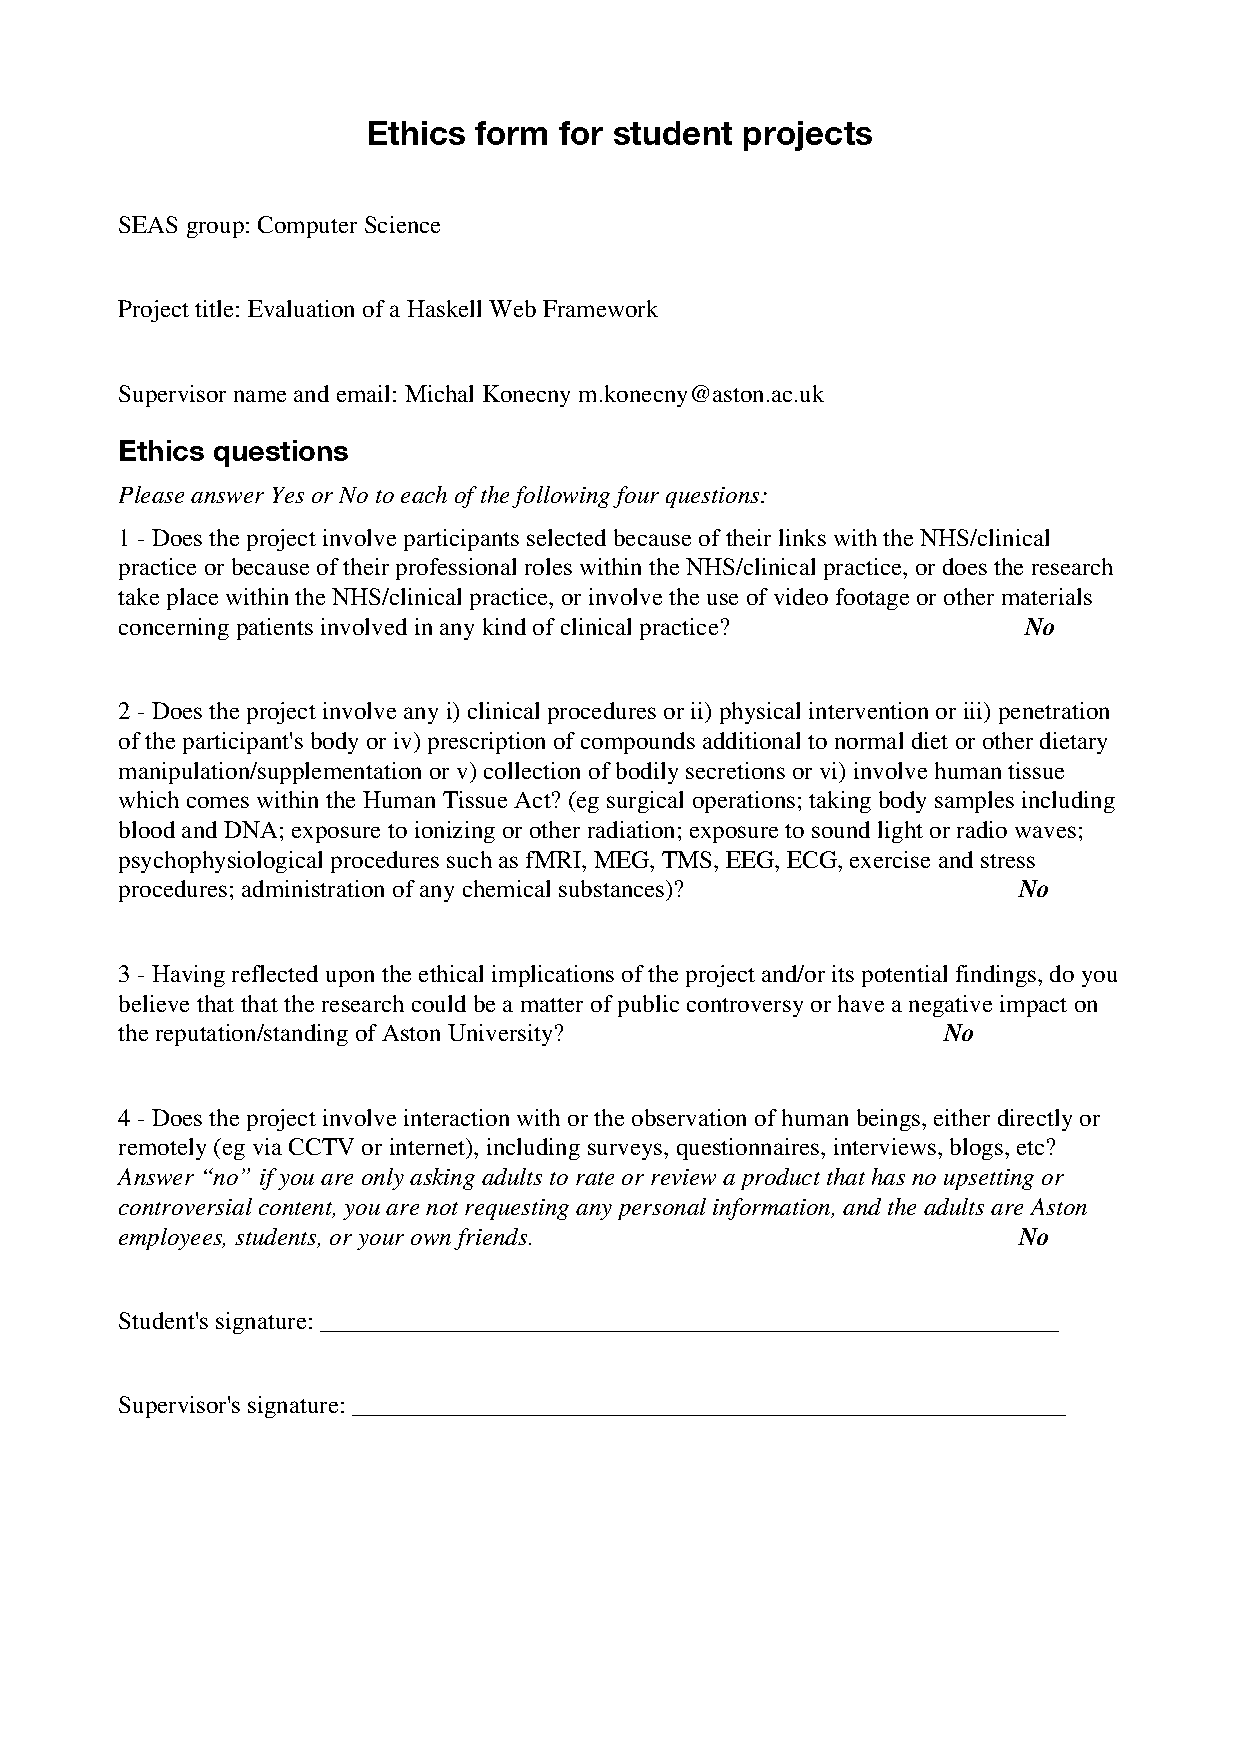
\includepdf[pages=1]{pdf_documents/seas-ethics-student-project-CS-FYP.pdf}


\end{appendices}

\end{document}
